\documentclass[10pt,a4paper]{article}
\usepackage[margin=1.8cm]{geometry}
\usepackage{graphicx}
\usepackage{caption}
\usepackage{placeins}
\usepackage[hidelinks]{hyperref}
\setlength{\textfloatsep}{8pt plus 2pt minus 2pt}
\captionsetup{font=small,skip=5pt,labelfont=bf}
\title{Supplementary Map Atlas\\CE634 Urban Big Data --- Assignment 1}
\author{ZHANG Ziqi / 24111604R}
\date{}
\begin{document}
\maketitle
\section{Spatial Demand}
The eight hotspot maps show completed-trip pickup and dropoff counts by TLC Taxi Zone. Zone 265 (Outside of NYC) is included in counts but has no drawable polygon.
\begin{figure}[!htbp]
\centering
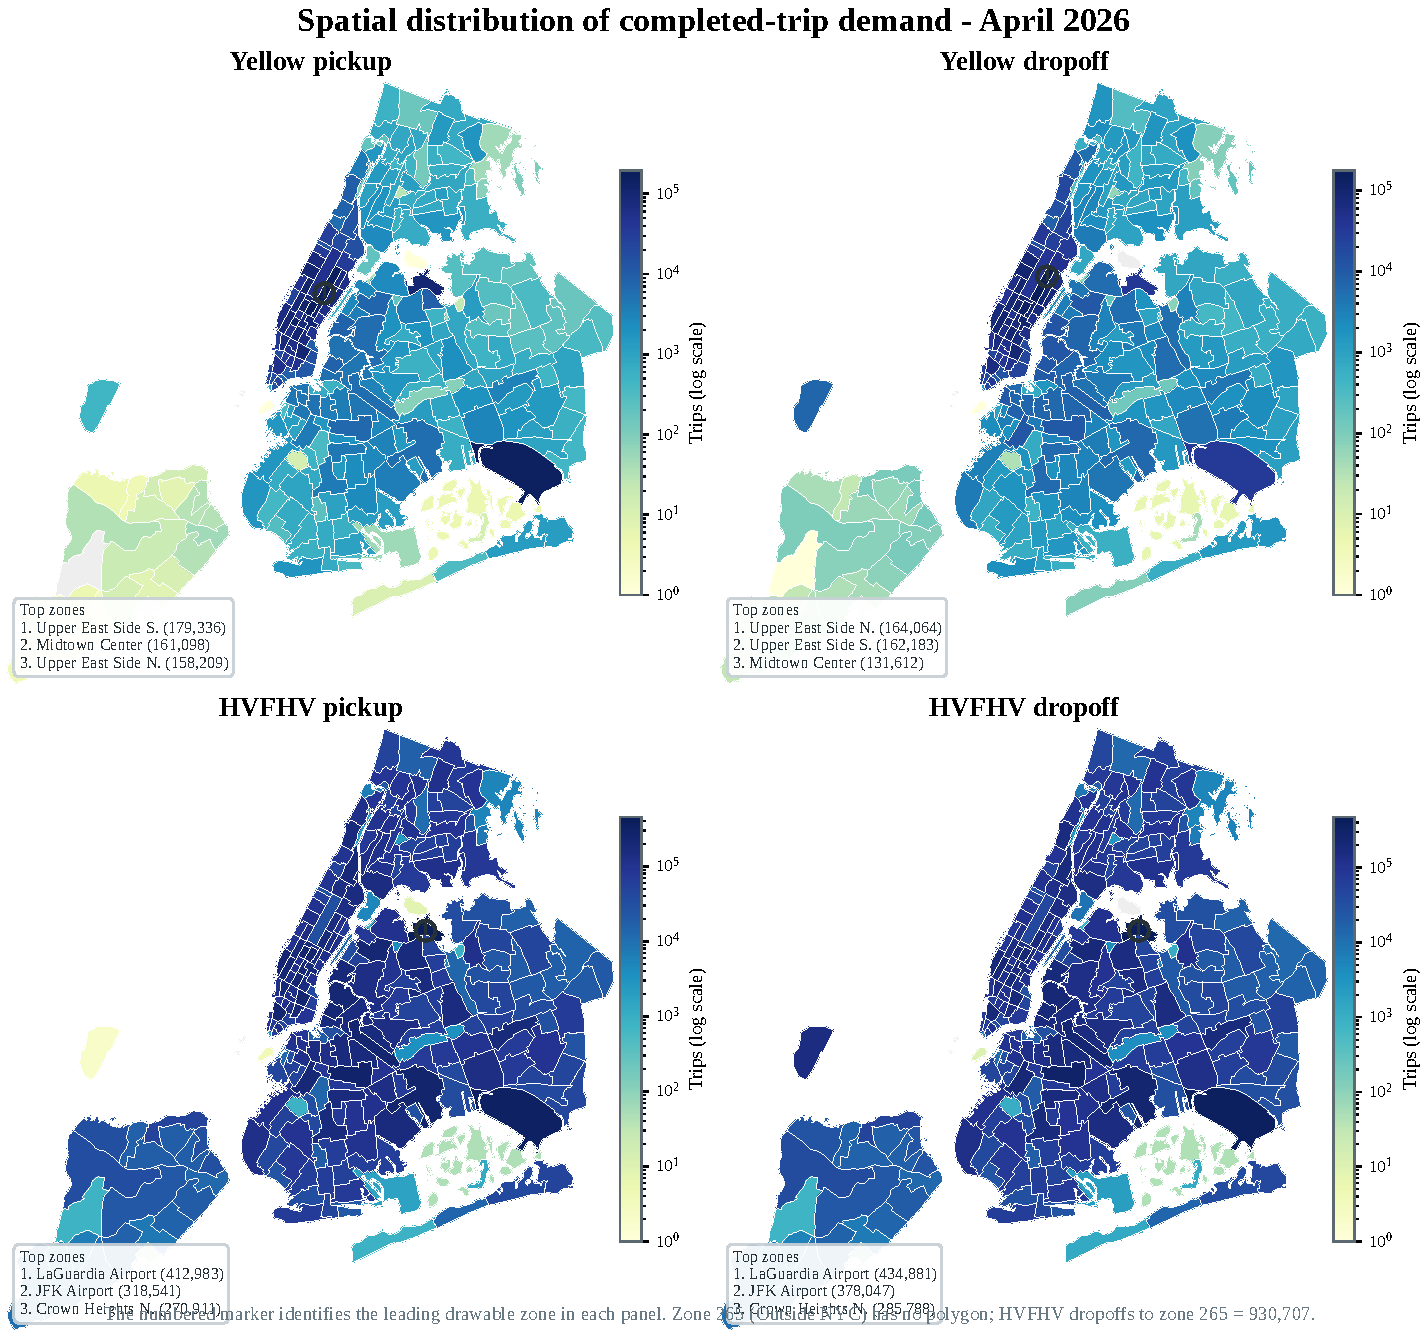
\includegraphics[width=.96\linewidth]{04_Results/paper_figures/main/fig2_spatial_demand_april.pdf}
\caption{\textbf{Task 2.1 hotspot maps for April 2026.} The four panels show Yellow Taxi origins, Yellow Taxi destinations, HVFHV origins, and HVFHV destinations. Each panel lists its three leading drawable zones and marks the highest-count drawable zone directly on the map. Yellow Taxi demand is strongly Manhattan-centered, whereas HVFHV demand is more geographically distributed and shows strong airport activity. Zone 265 is counted in the analysis but cannot be colored because no polygon is provided.}
\label{fig:spatial_apr}
\end{figure}

\begin{figure}[!htbp]
\centering
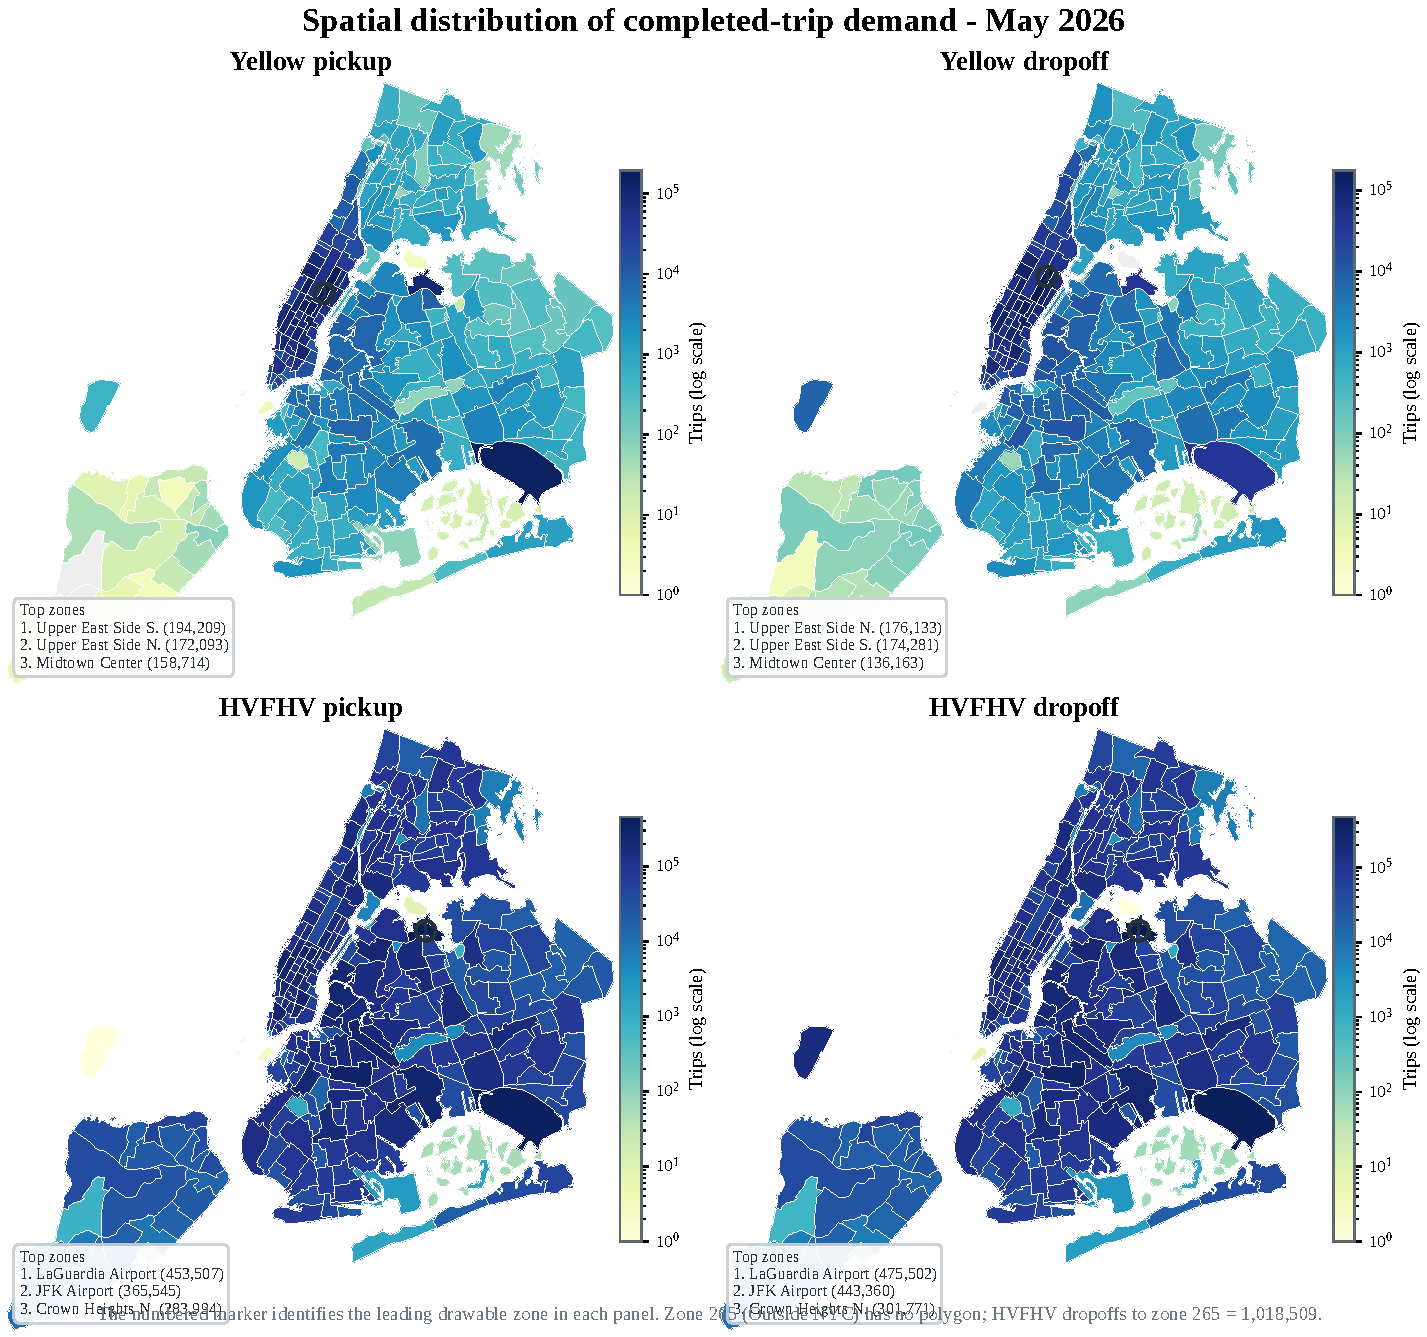
\includegraphics[width=.96\linewidth]{04_Results/paper_figures/main/fig3_spatial_demand_may.pdf}
\caption{\textbf{Task 2.1 hotspot maps for May 2026.} The four panels show Yellow Taxi origins, Yellow Taxi destinations, HVFHV origins, and HVFHV destinations. The same service/measure scales are used as in April to support month-to-month comparison. The main spatial pattern remains stable, while several airport and Manhattan zones record higher counts.}
\label{fig:spatial_may}
\end{figure}

\clearpage
\section{Detailed OD and Pooling Maps}
OD arrows connect zone centroids, not driven routes. Gray areas in zone-level pooling maps indicate insufficient sample rather than zero.
\begingroup
\captionsetup{font=footnotesize,skip=3pt,hypcap=false}
\setlength{\abovecaptionskip}{3pt}
\setlength{\belowcaptionskip}{0pt}

\subsection{Detailed directed OD rankings}
The following compact pages show the ten leading directed OD pairs by trip volume and by aggregate passenger spending for each service and month. The original map images are unchanged; only their placement in the supplement is condensed.

\begin{center}
\centering
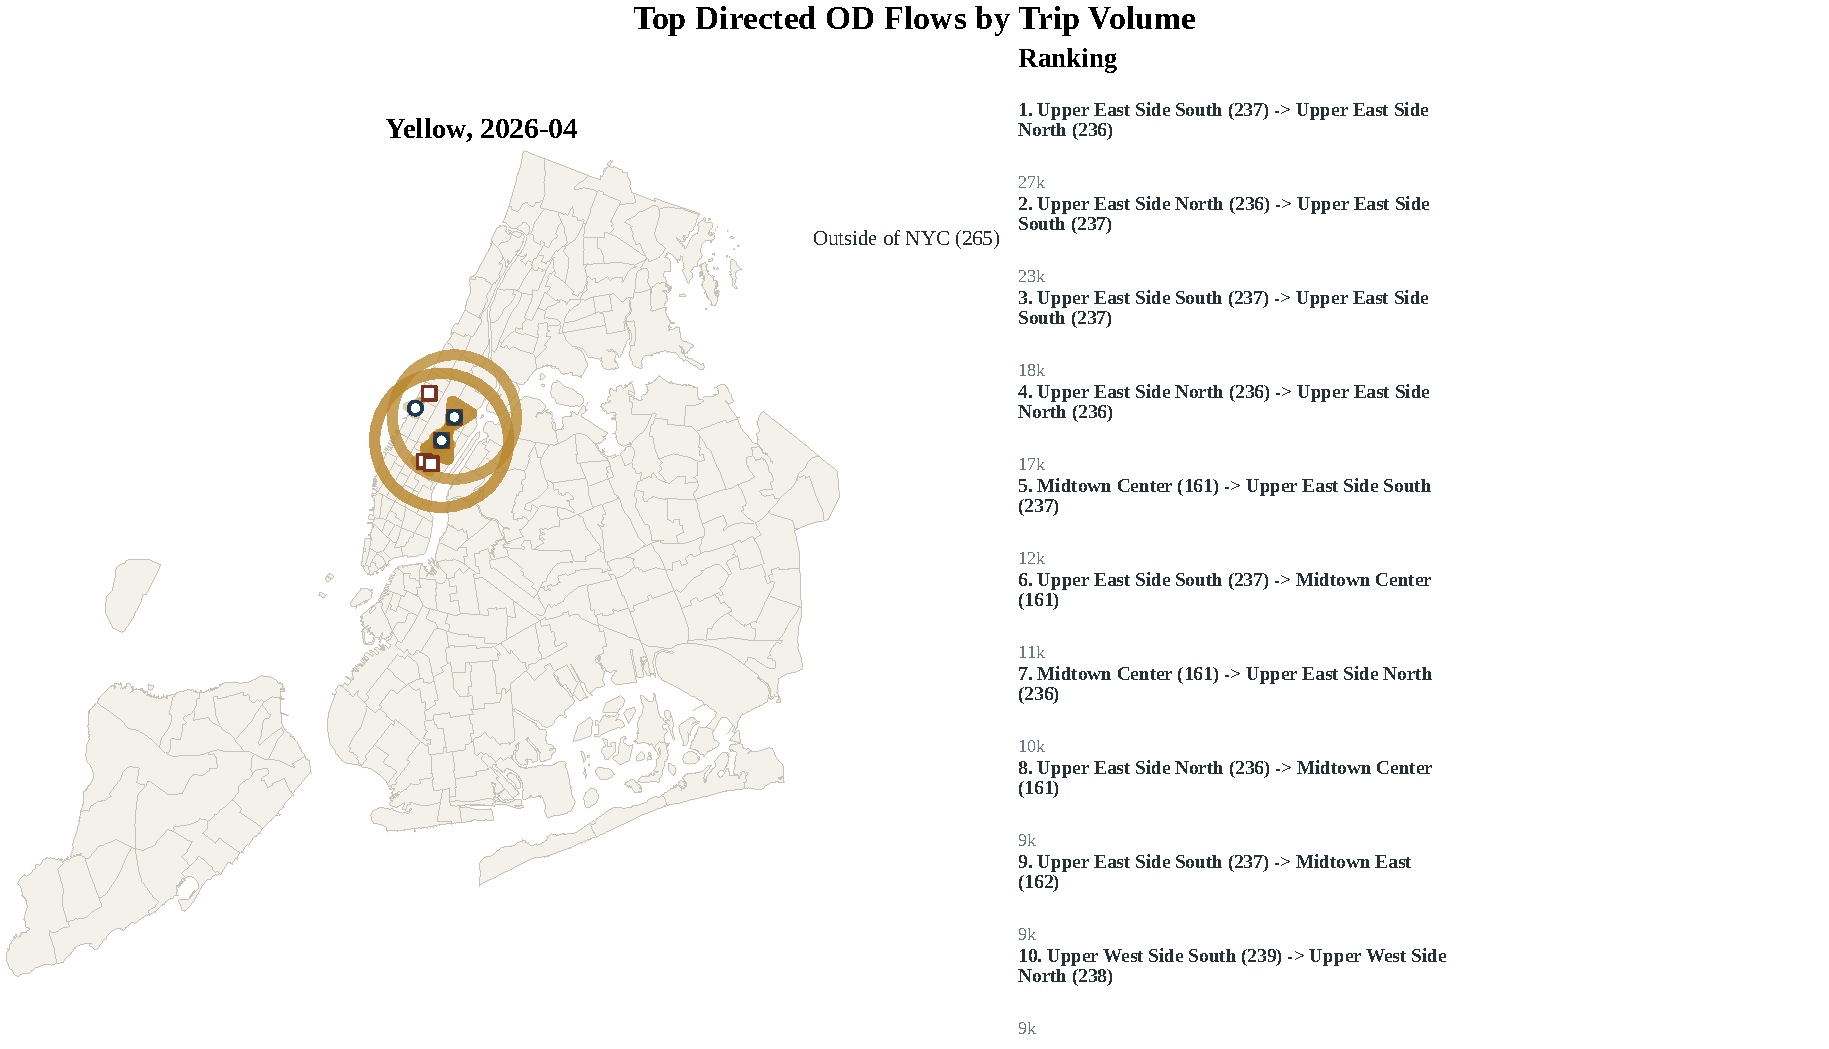
\includegraphics[height=.265\textheight,width=.98\linewidth,keepaspectratio]{04_Results/report_figures/appendix/task2_od_volume_2026-04_yellow.pdf}\par\vspace{0.2em}
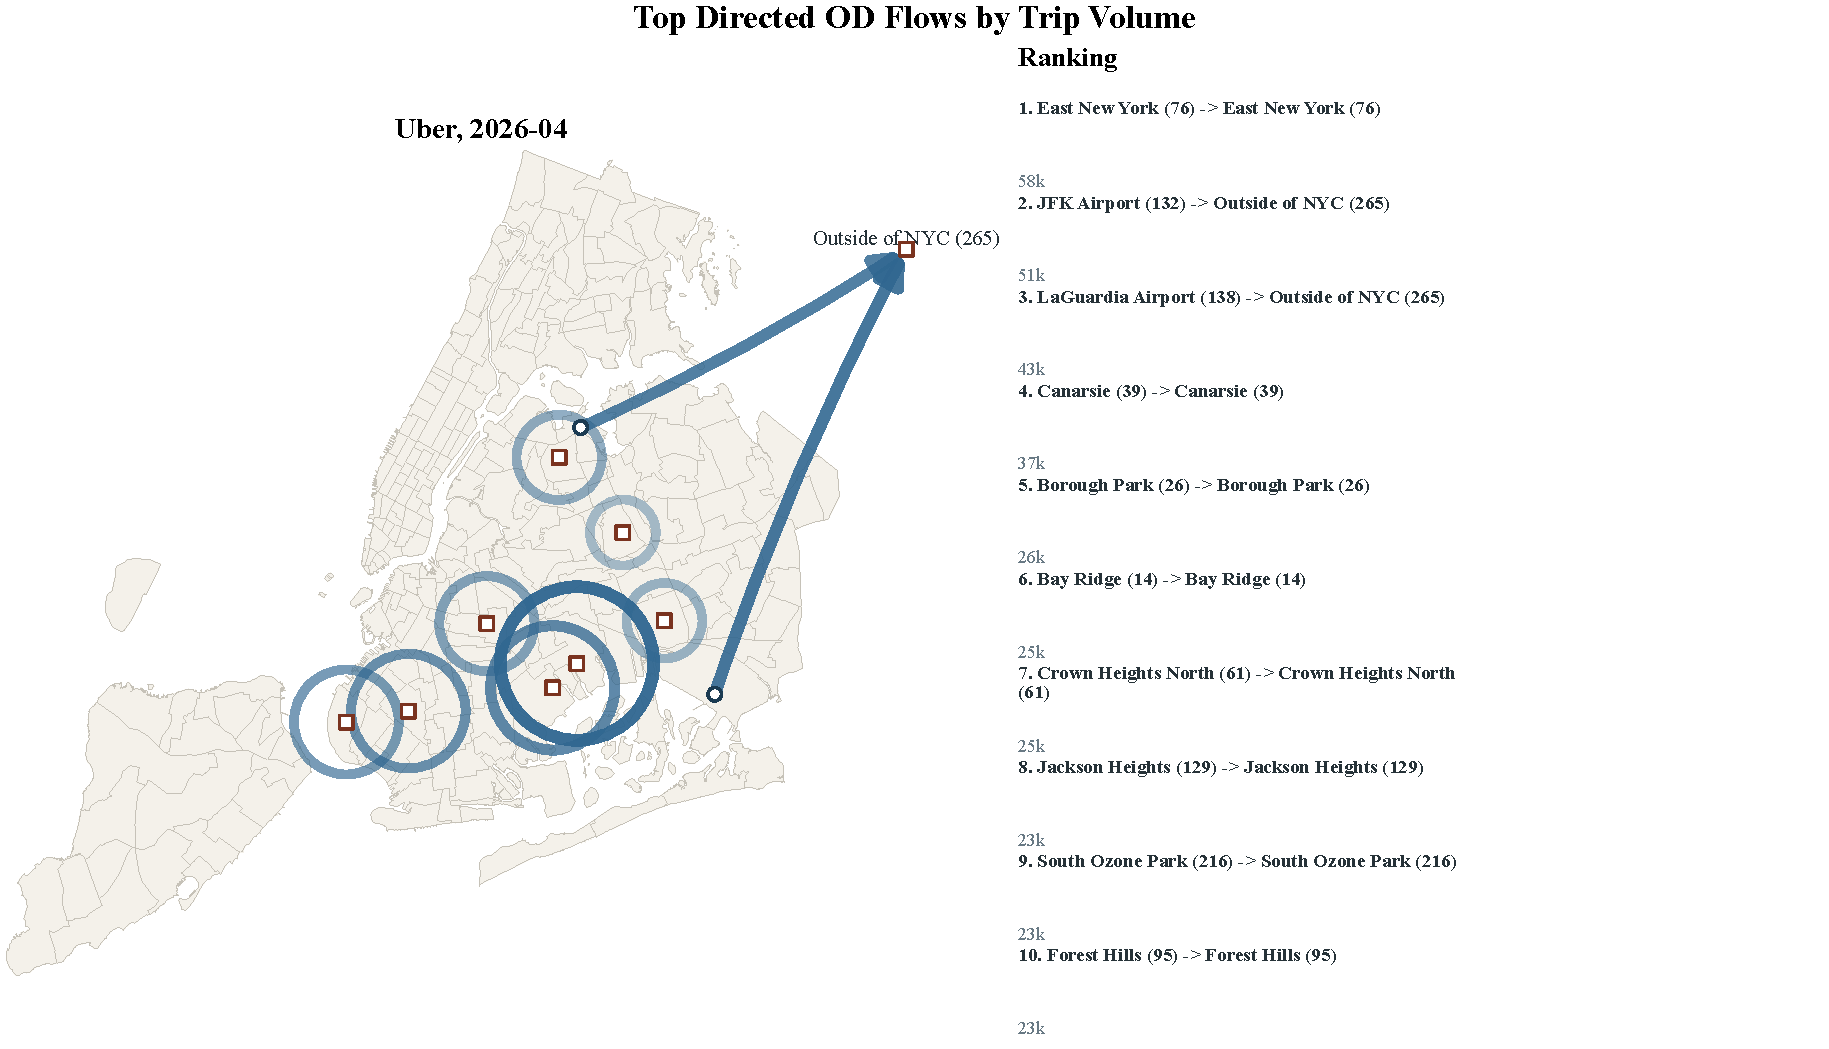
\includegraphics[height=.265\textheight,width=.98\linewidth,keepaspectratio]{04_Results/report_figures/appendix/task2_od_volume_2026-04_uber.pdf}\par\vspace{0.2em}
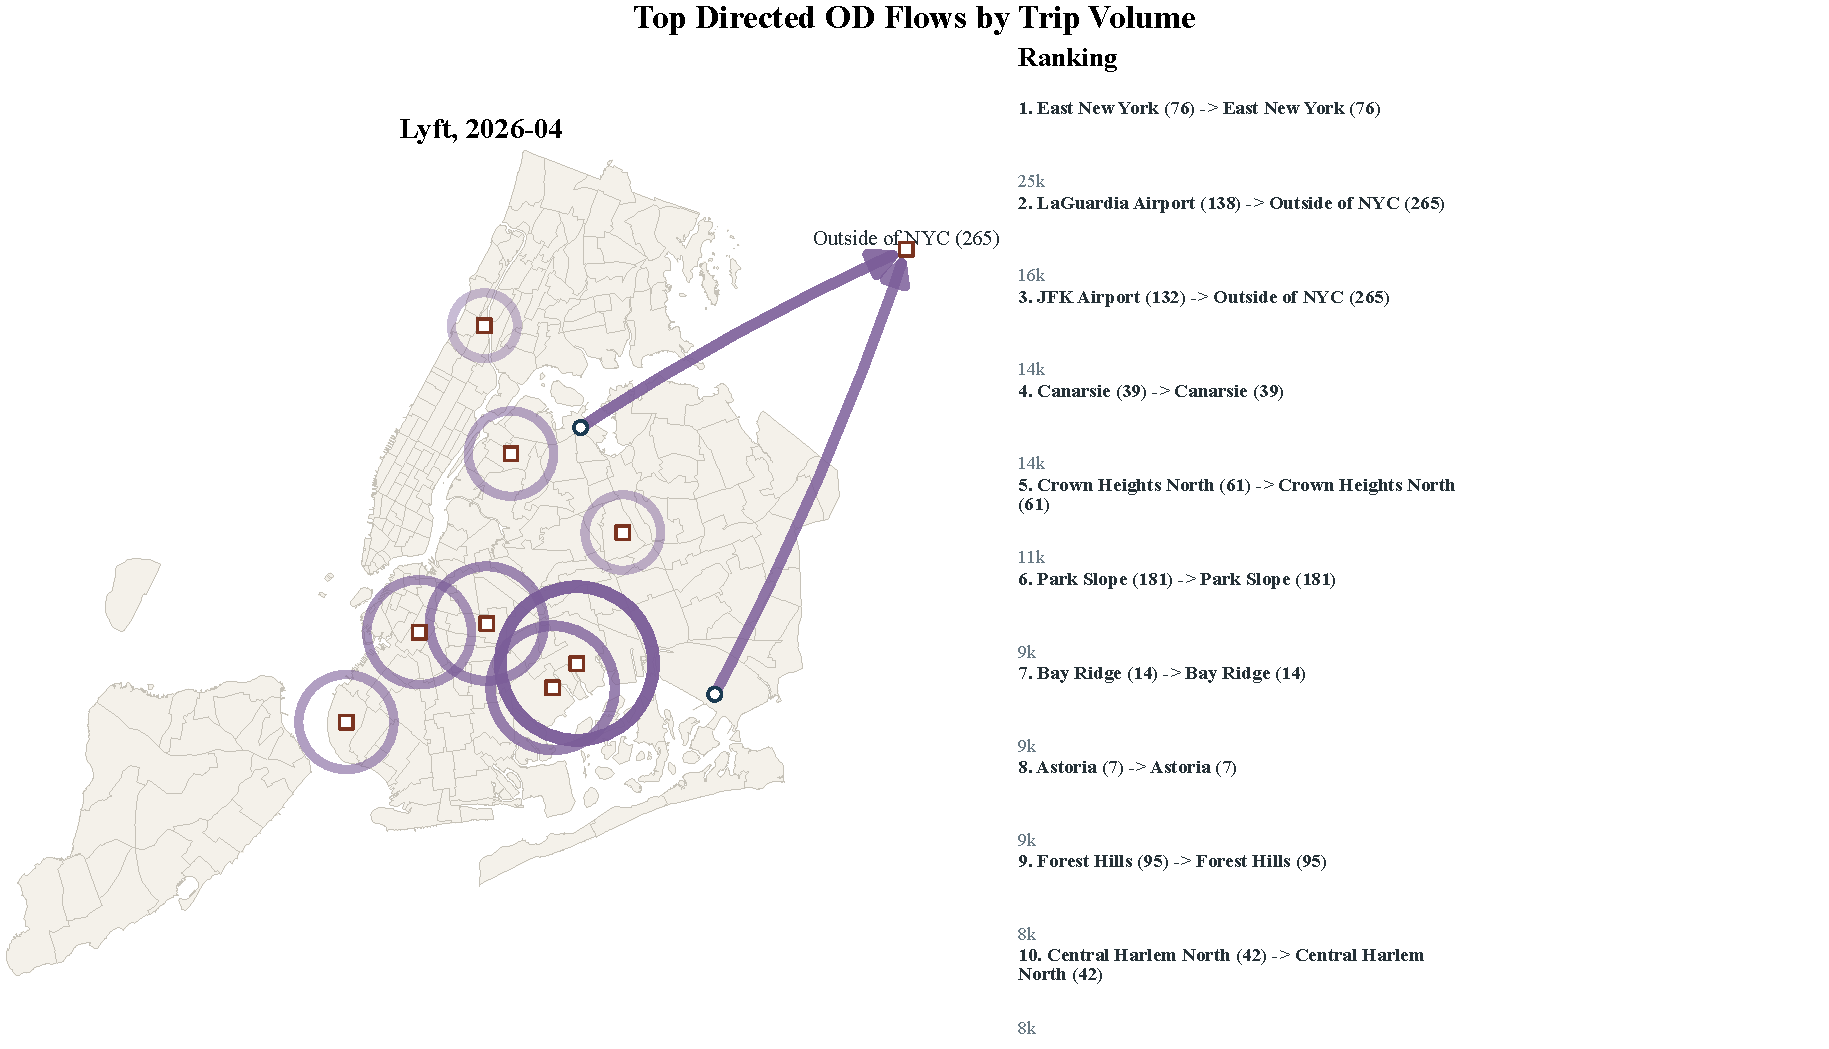
\includegraphics[height=.265\textheight,width=.98\linewidth,keepaspectratio]{04_Results/report_figures/appendix/task2_od_volume_2026-04_lyft.pdf}
\captionof{figure}{Top ten OD flows by trip volume, 2026-04. Panels from top to bottom: Yellow Taxi, Uber, and Lyft.}
\end{center}
\clearpage

\begin{center}
\centering
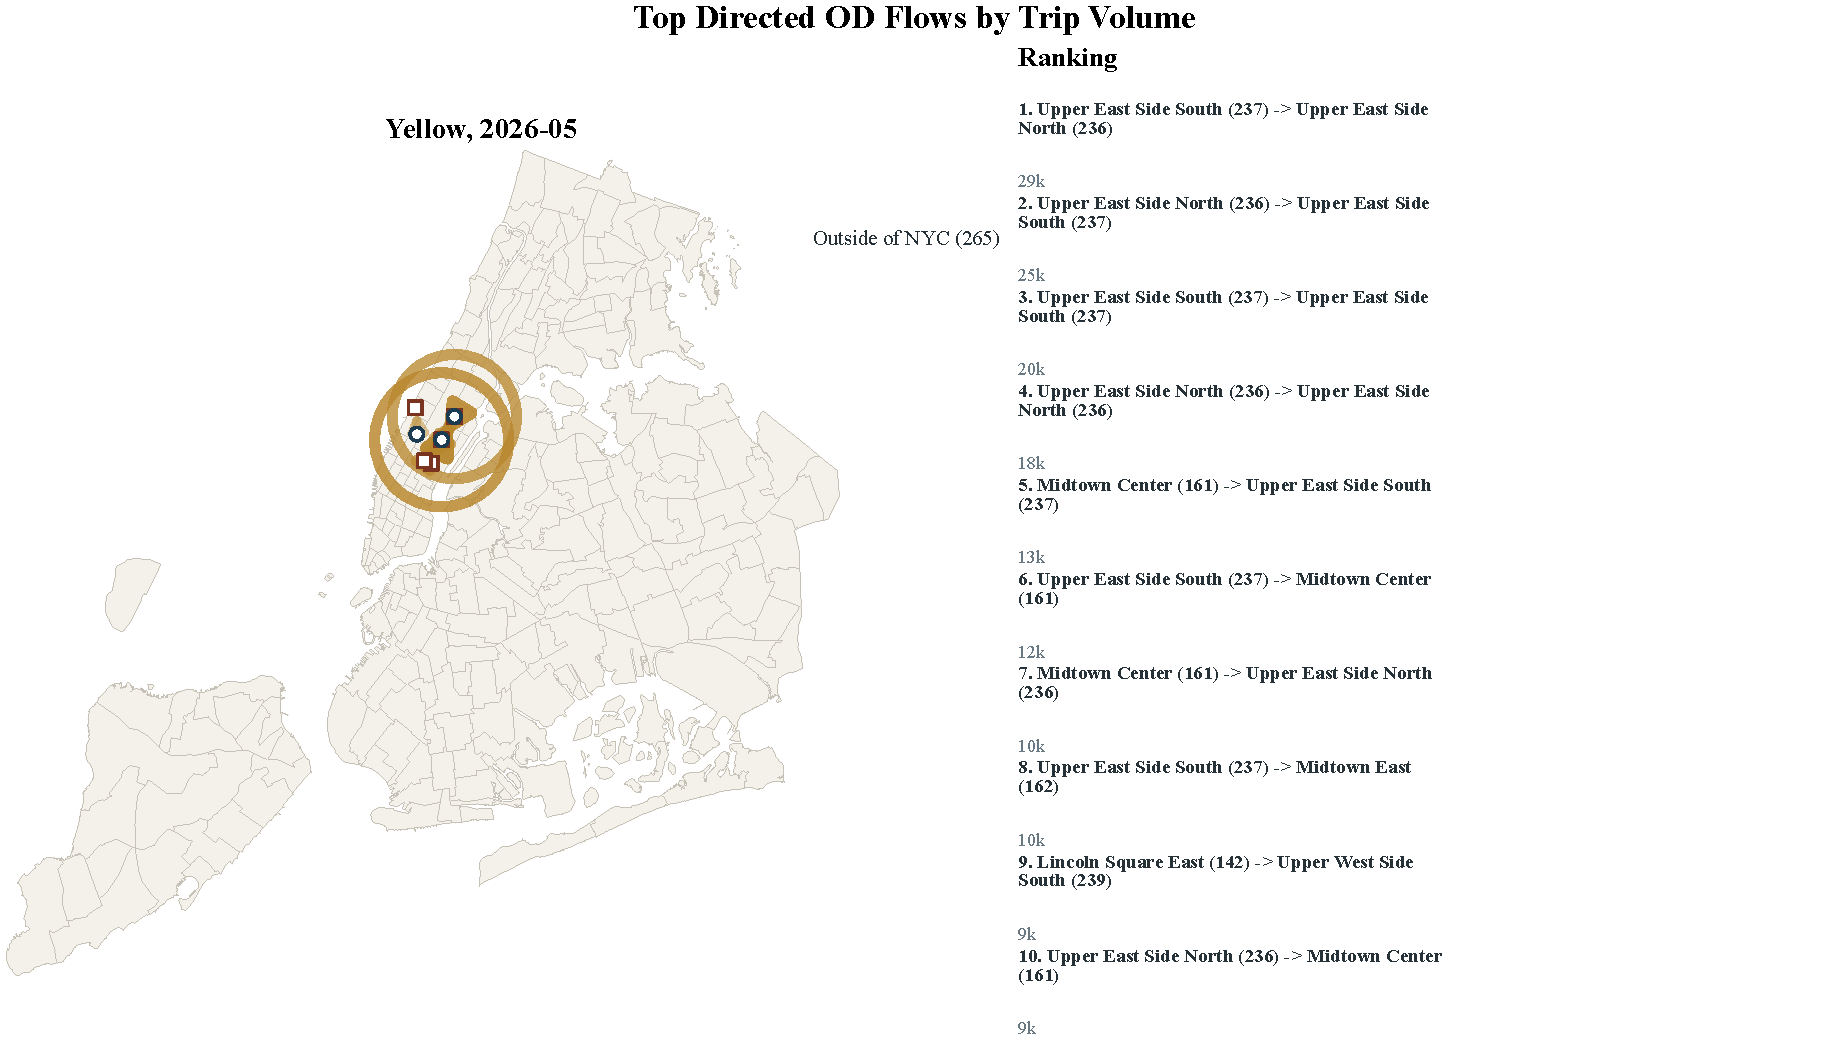
\includegraphics[height=.265\textheight,width=.98\linewidth,keepaspectratio]{04_Results/report_figures/appendix/task2_od_volume_2026-05_yellow.pdf}\par\vspace{0.2em}
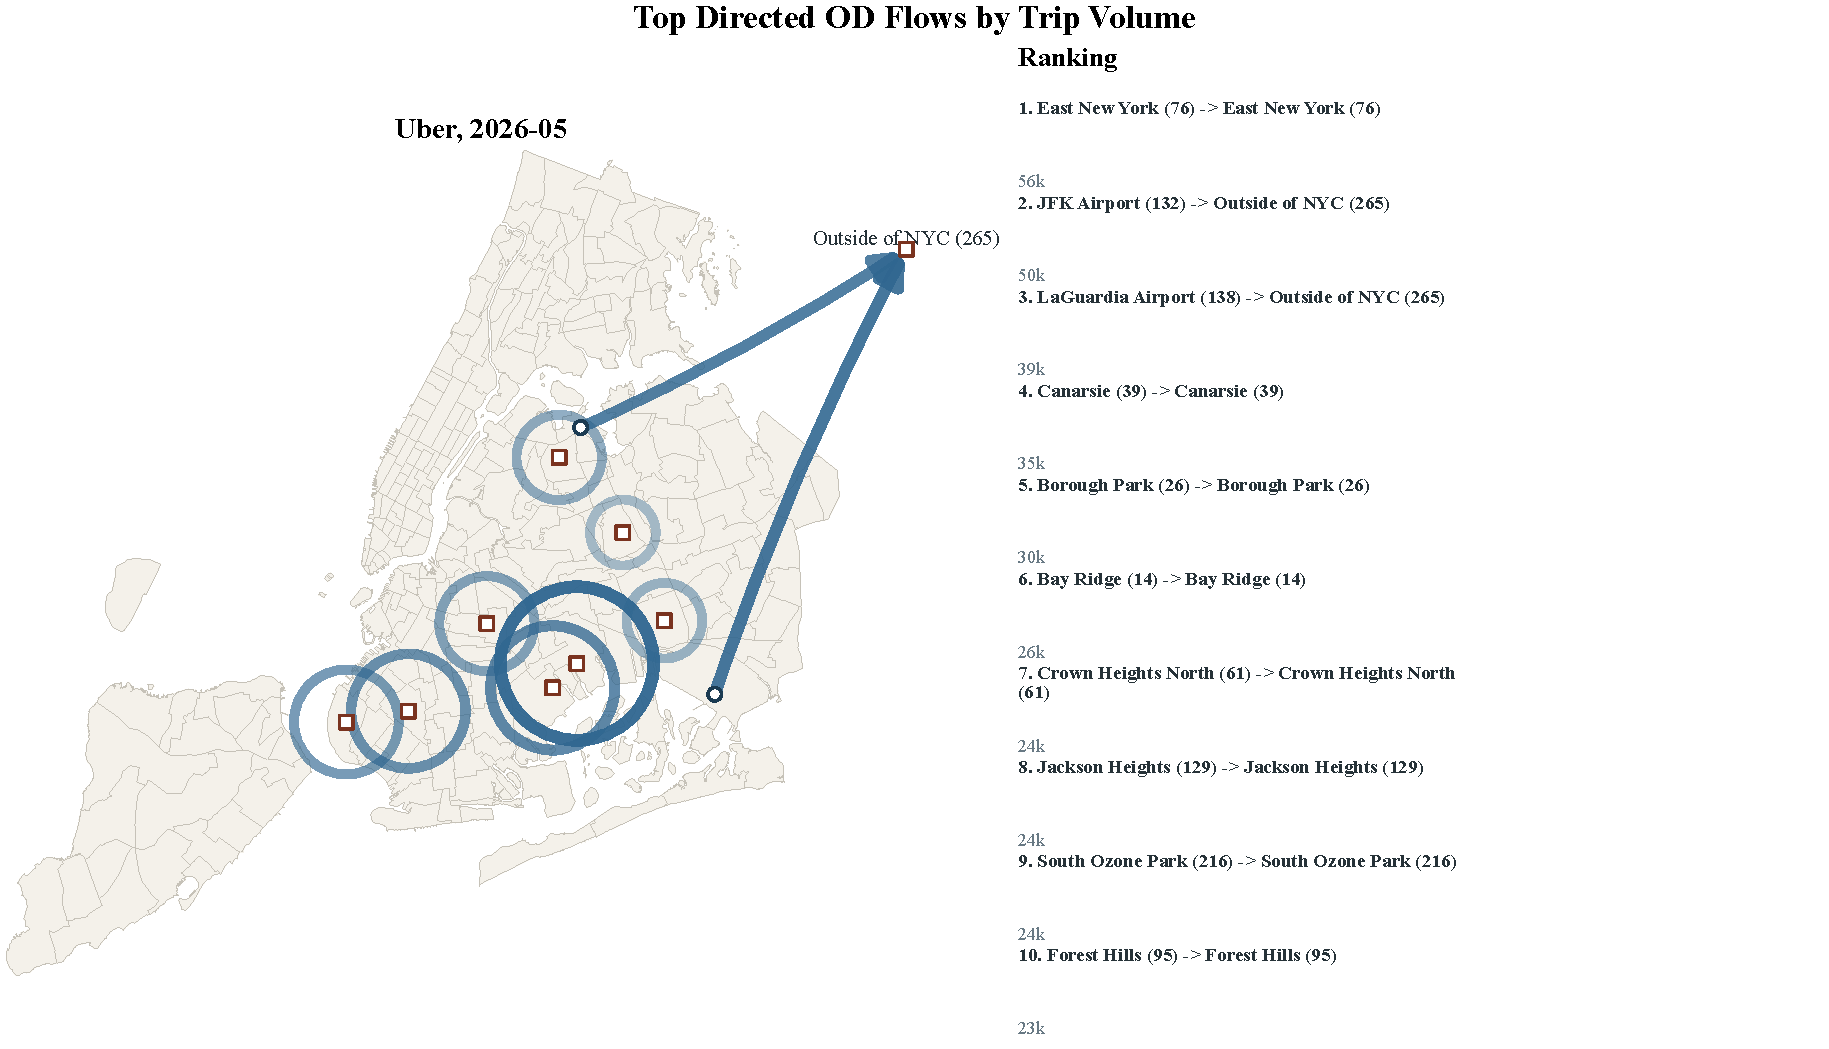
\includegraphics[height=.265\textheight,width=.98\linewidth,keepaspectratio]{04_Results/report_figures/appendix/task2_od_volume_2026-05_uber.pdf}\par\vspace{0.2em}
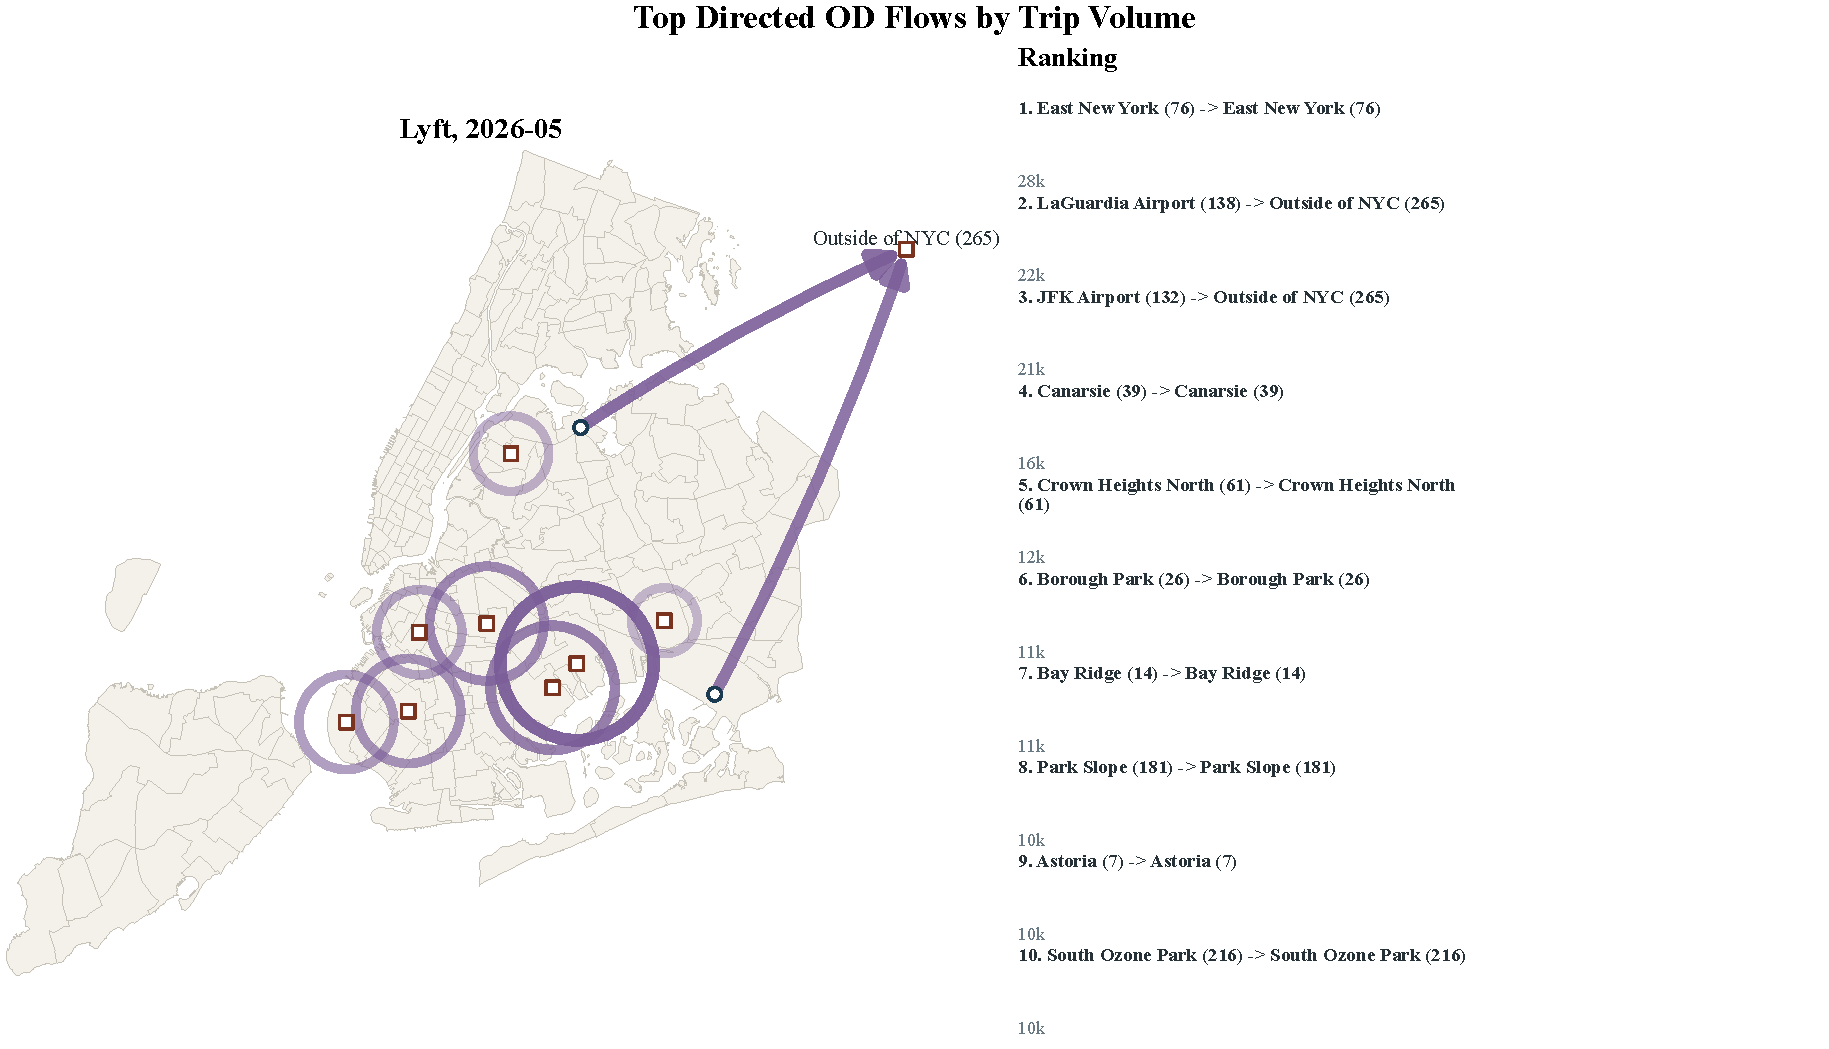
\includegraphics[height=.265\textheight,width=.98\linewidth,keepaspectratio]{04_Results/report_figures/appendix/task2_od_volume_2026-05_lyft.pdf}
\captionof{figure}{Top ten OD flows by trip volume, 2026-05. Panels from top to bottom: Yellow Taxi, Uber, and Lyft.}
\end{center}
\clearpage

\begin{center}
\centering
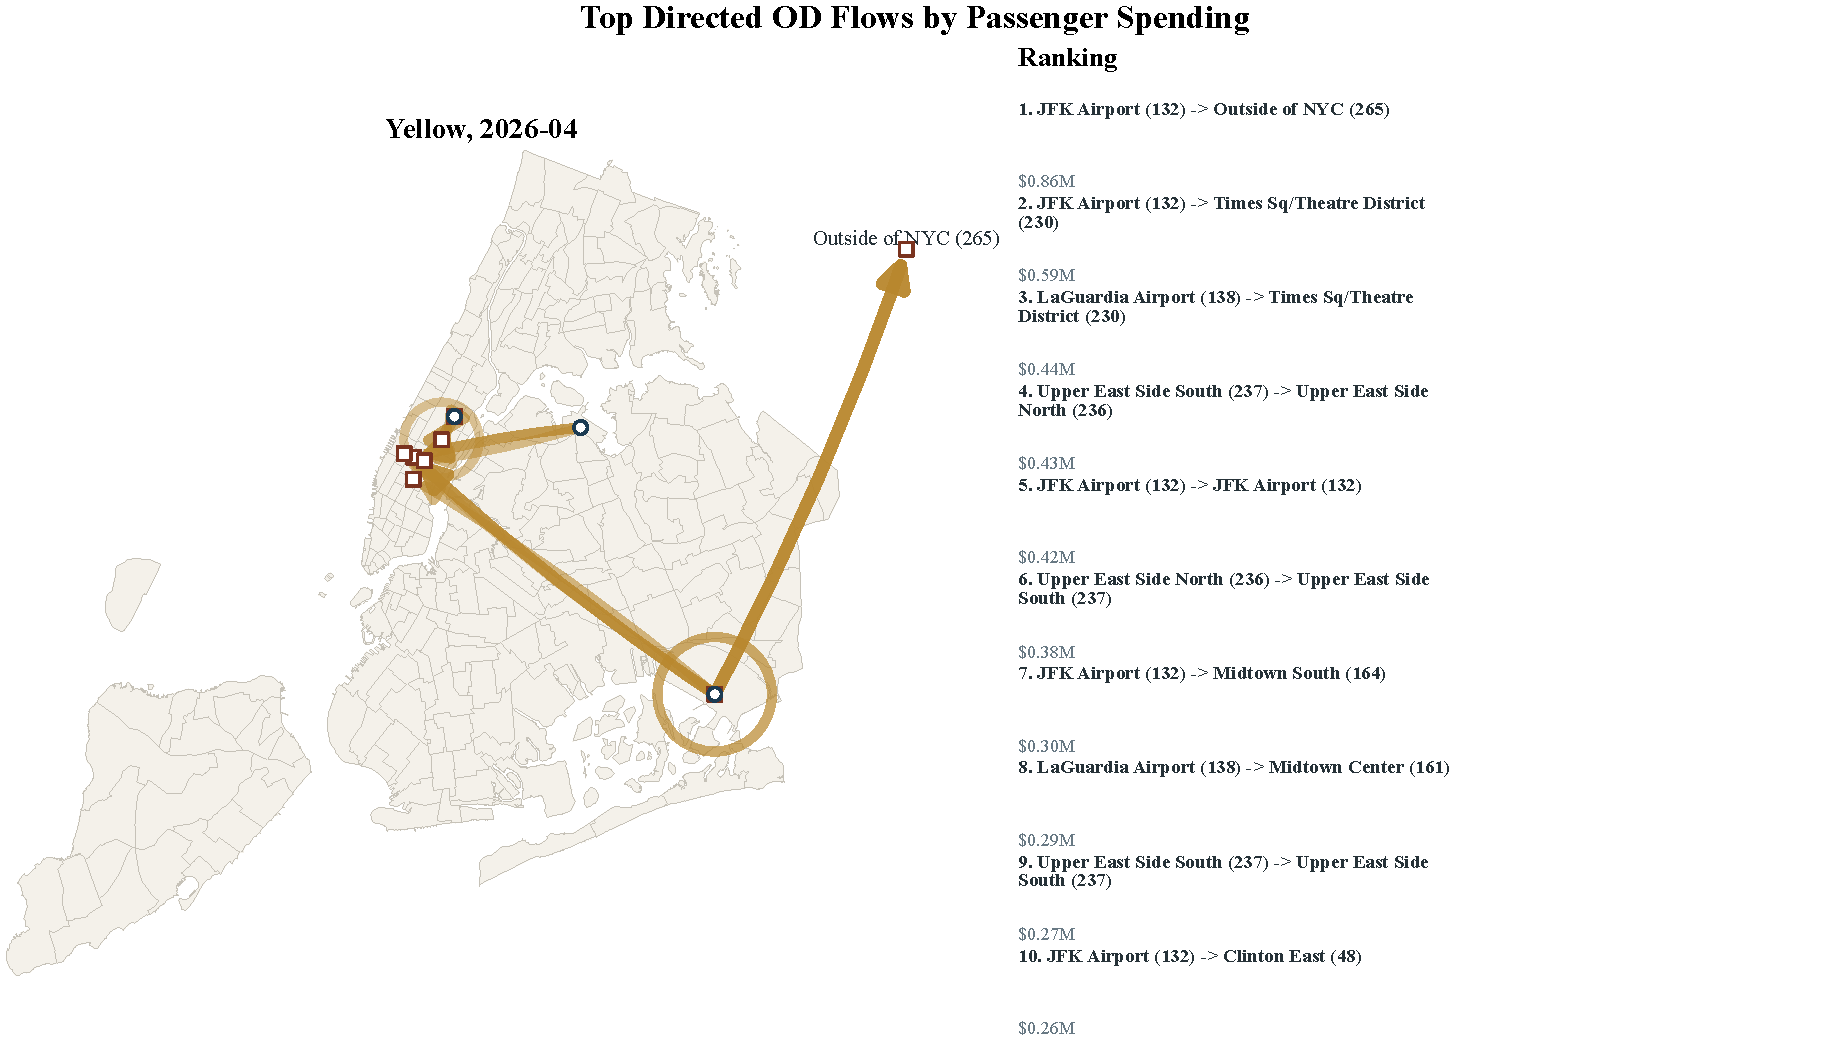
\includegraphics[height=.265\textheight,width=.98\linewidth,keepaspectratio]{04_Results/report_figures/appendix/task2_od_spending_2026-04_yellow.pdf}\par\vspace{0.2em}
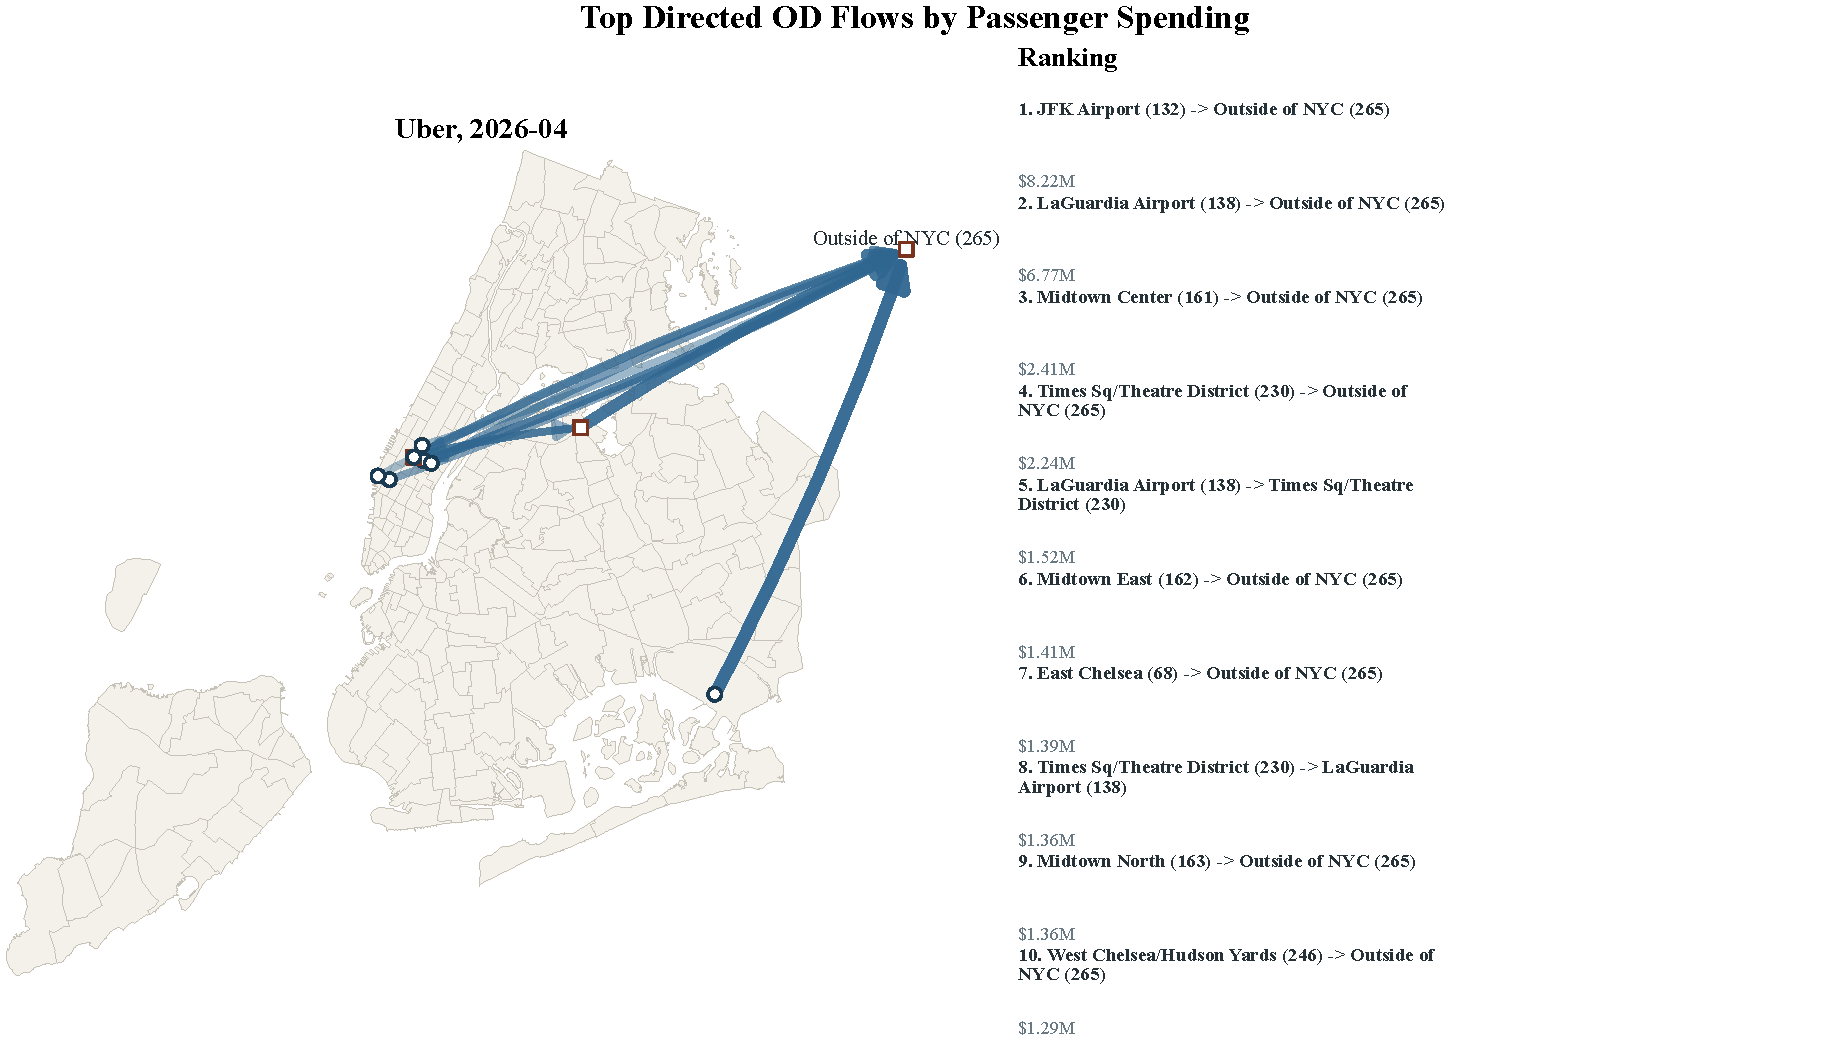
\includegraphics[height=.265\textheight,width=.98\linewidth,keepaspectratio]{04_Results/report_figures/appendix/task2_od_spending_2026-04_uber.pdf}\par\vspace{0.2em}
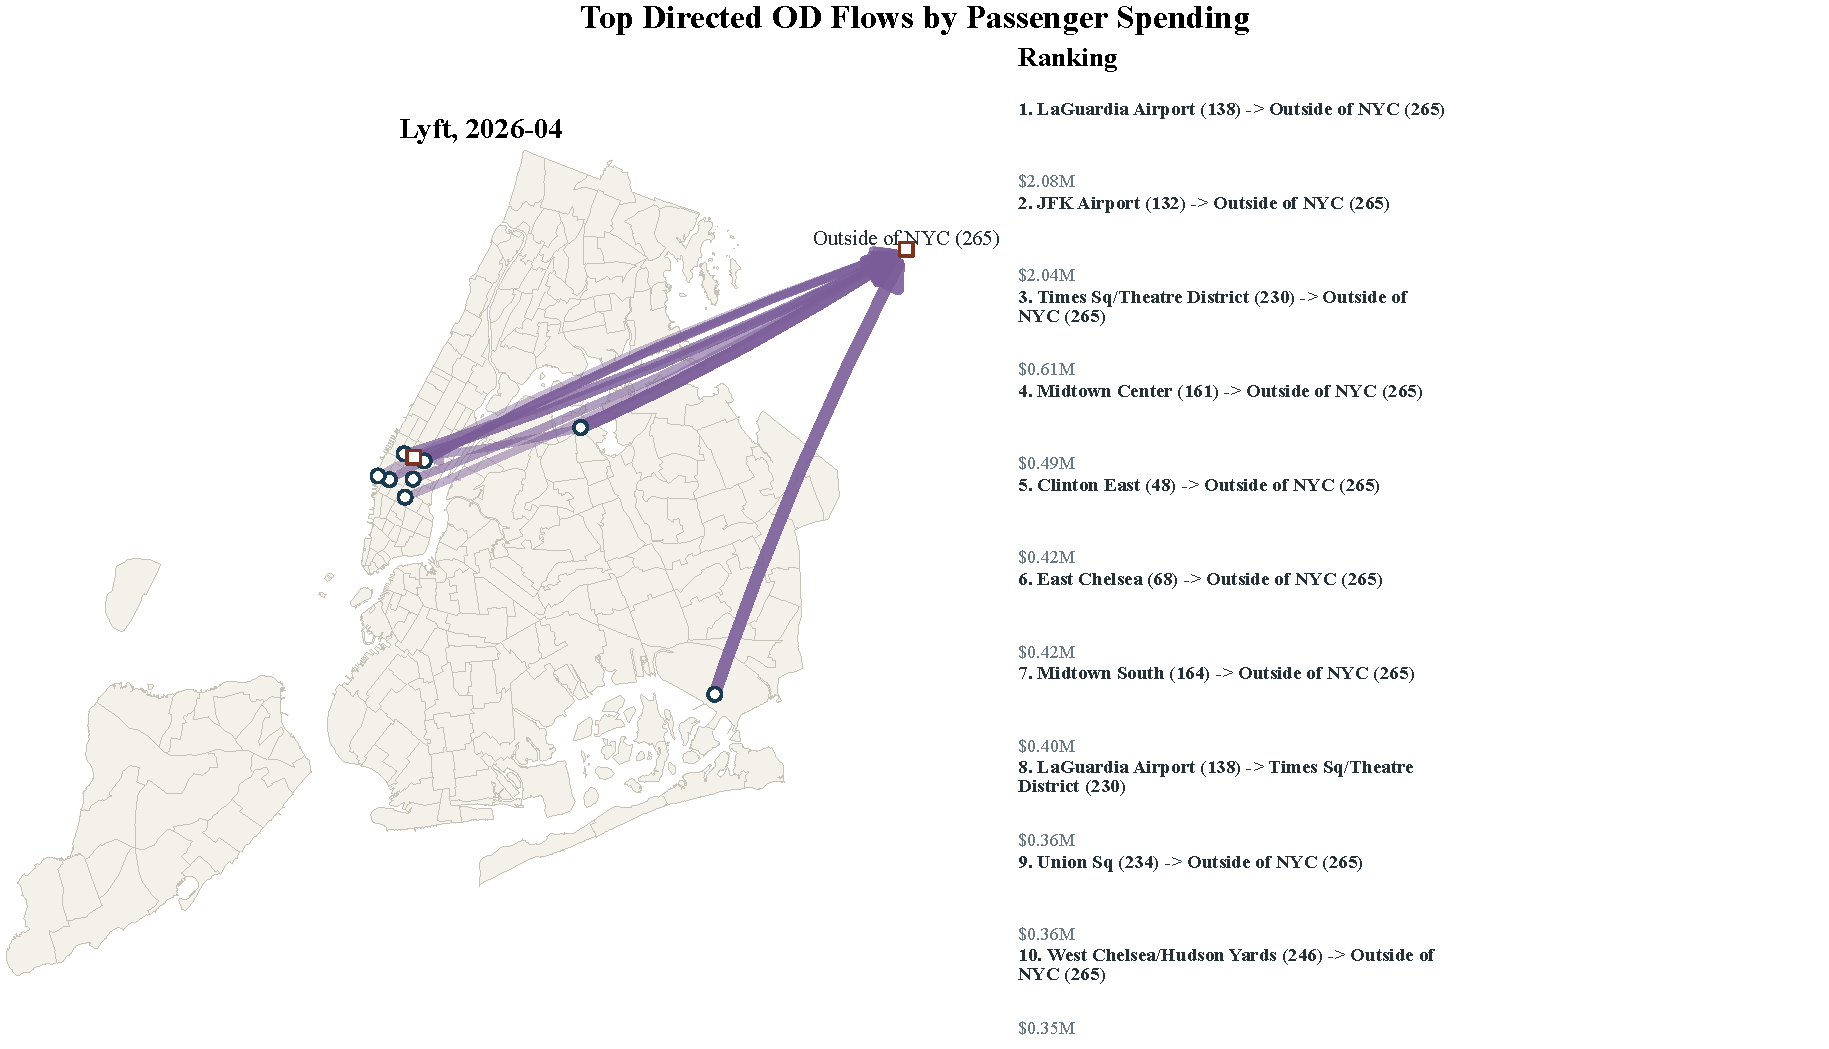
\includegraphics[height=.265\textheight,width=.98\linewidth,keepaspectratio]{04_Results/report_figures/appendix/task2_od_spending_2026-04_lyft.pdf}
\captionof{figure}{Top ten OD flows by aggregate passenger spending, 2026-04. Panels from top to bottom: Yellow Taxi, Uber, and Lyft.}
\end{center}
\clearpage

\begin{center}
\centering
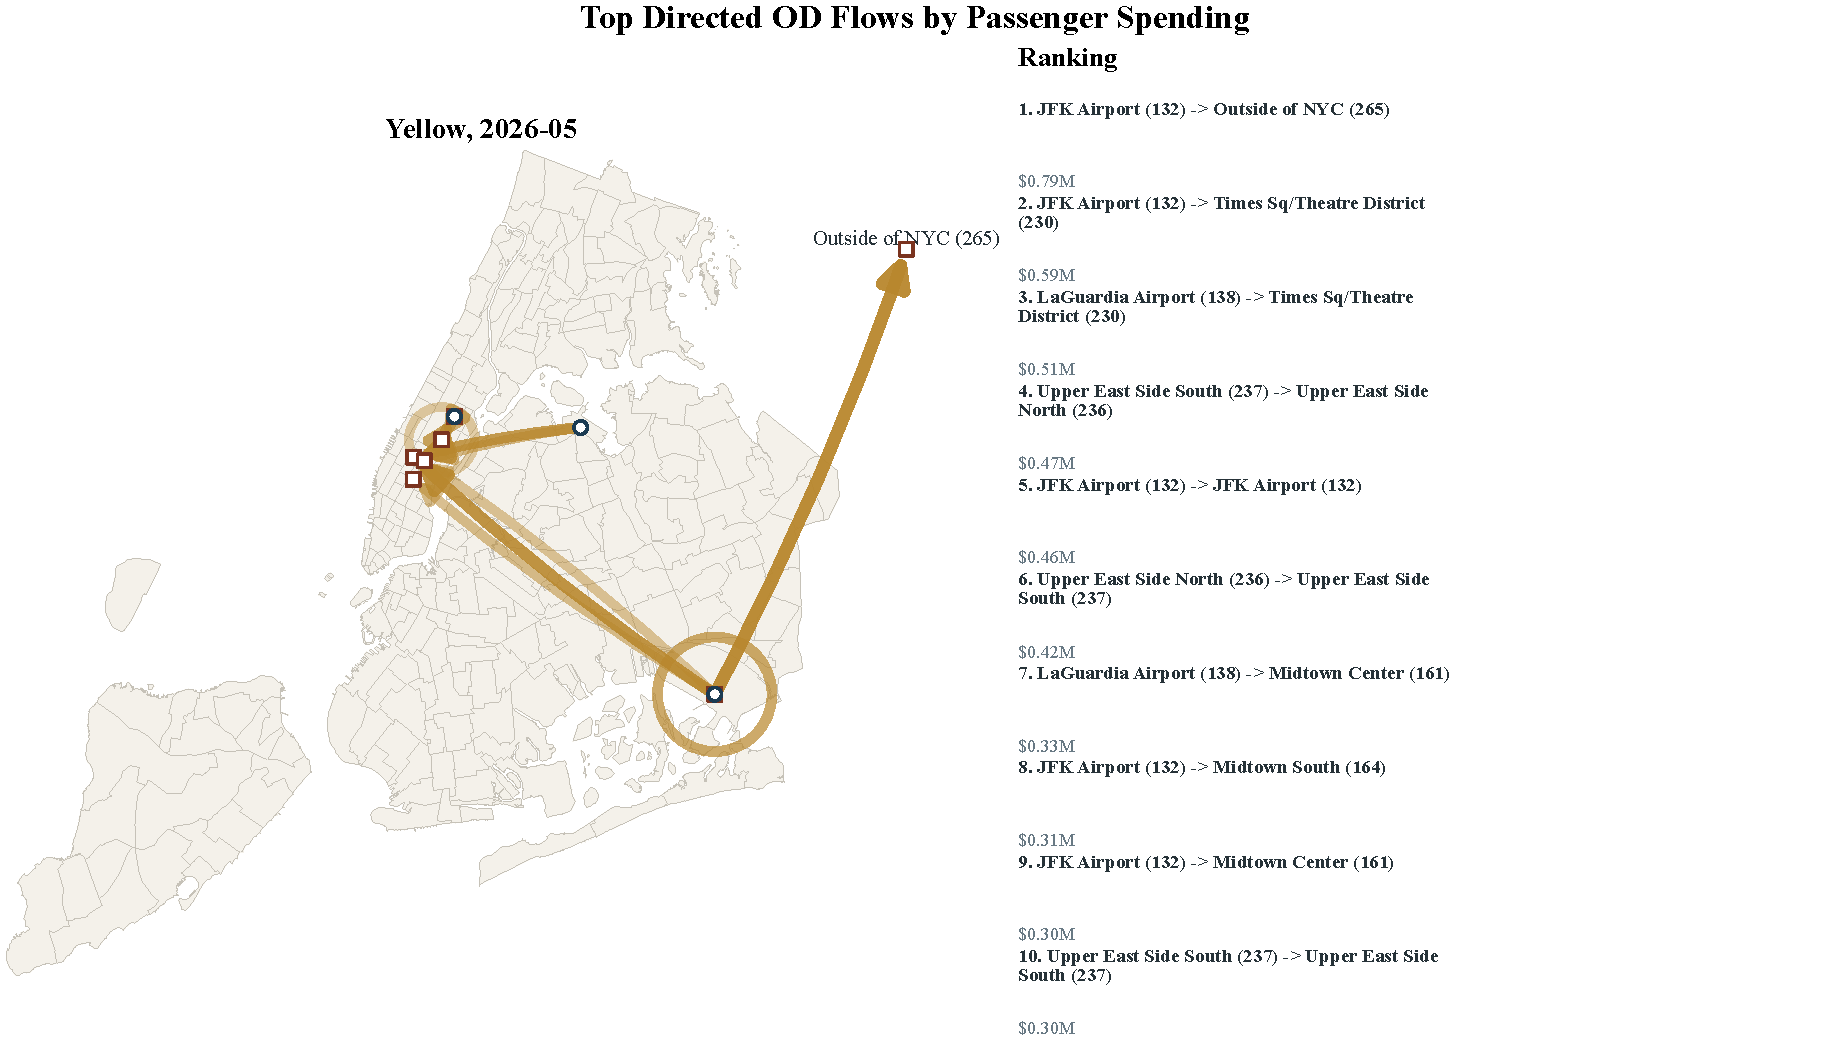
\includegraphics[height=.265\textheight,width=.98\linewidth,keepaspectratio]{04_Results/report_figures/appendix/task2_od_spending_2026-05_yellow.pdf}\par\vspace{0.2em}
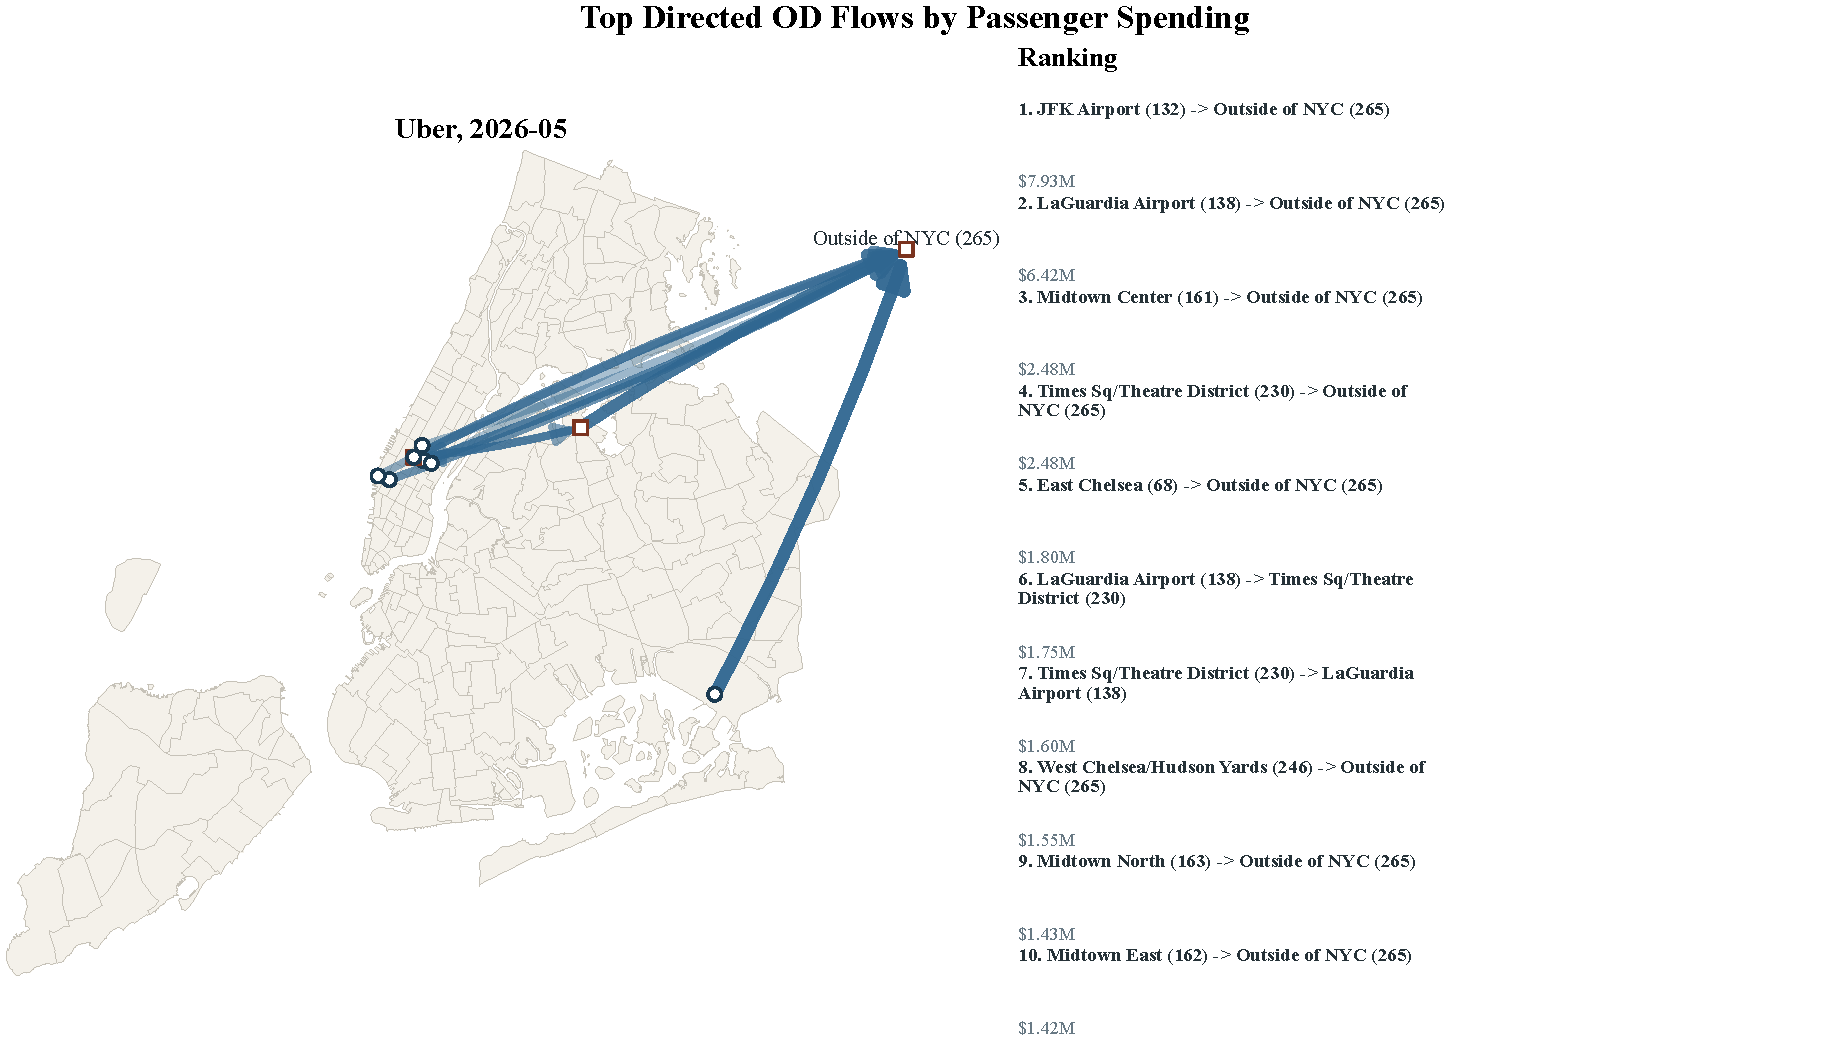
\includegraphics[height=.265\textheight,width=.98\linewidth,keepaspectratio]{04_Results/report_figures/appendix/task2_od_spending_2026-05_uber.pdf}\par\vspace{0.2em}
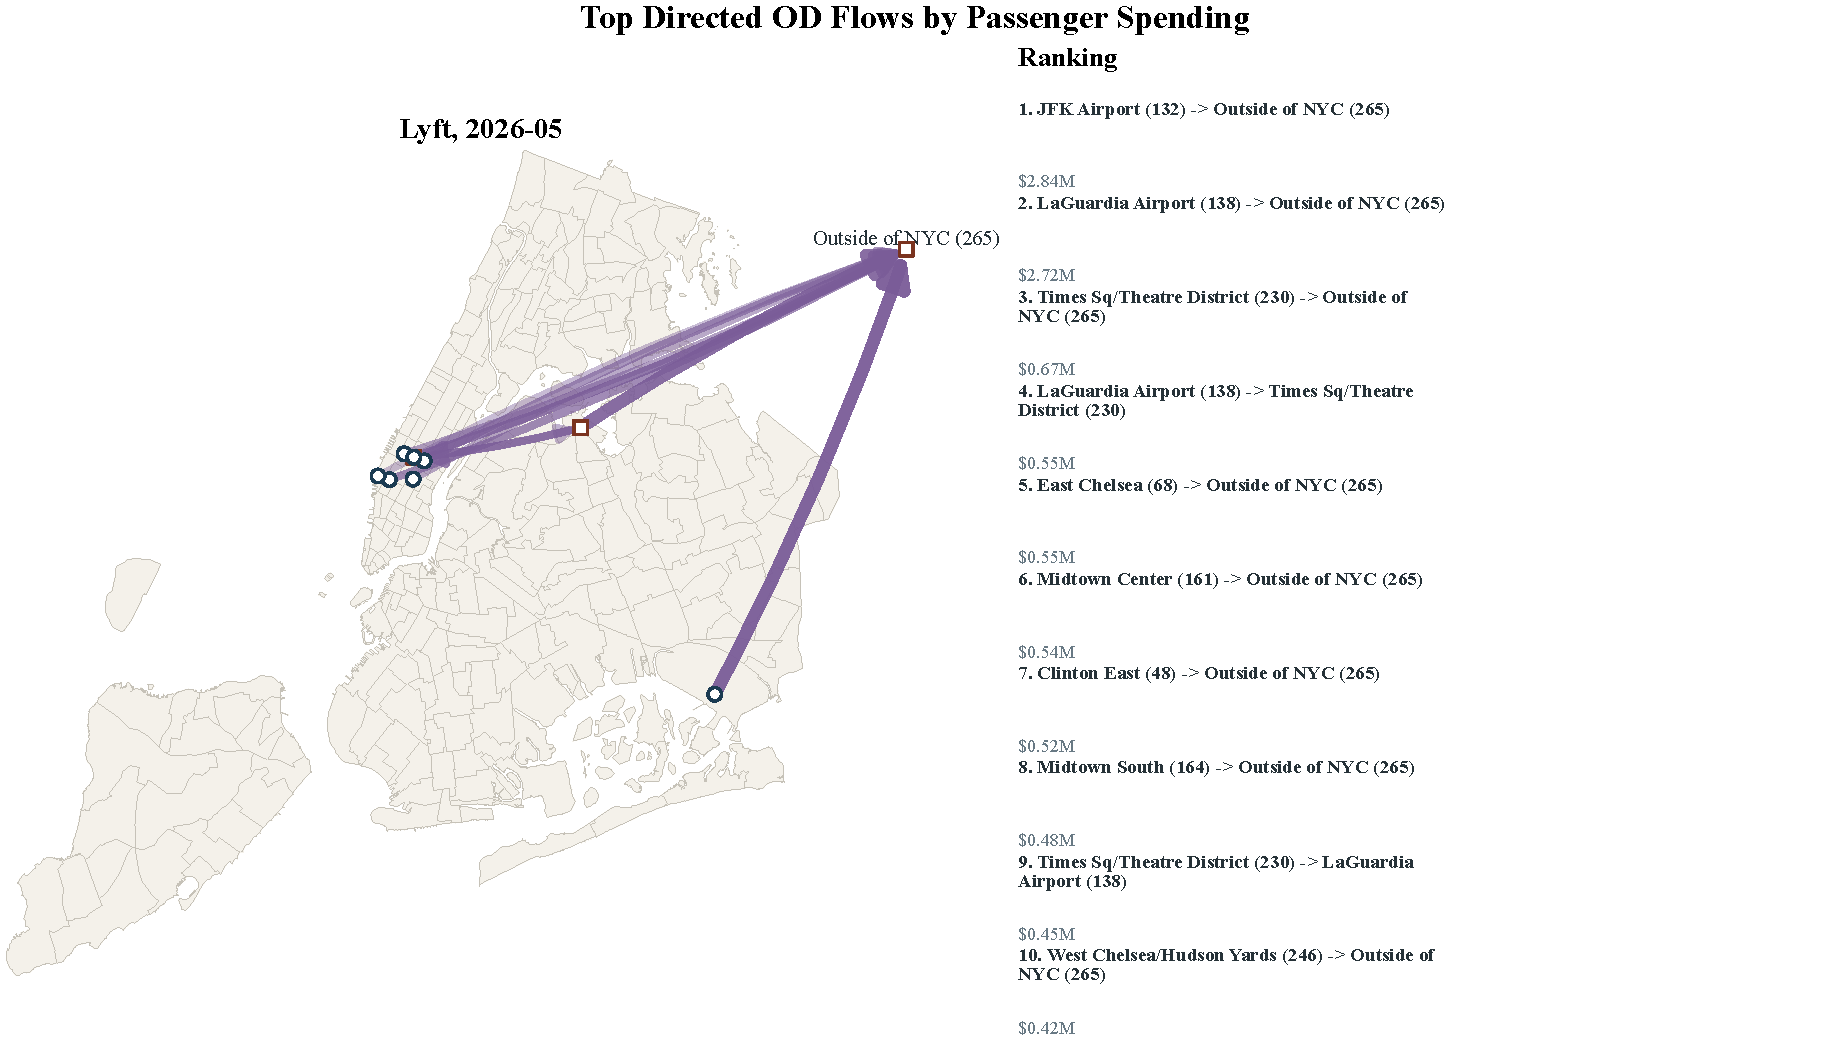
\includegraphics[height=.265\textheight,width=.98\linewidth,keepaspectratio]{04_Results/report_figures/appendix/task2_od_spending_2026-05_lyft.pdf}
\captionof{figure}{Top ten OD flows by aggregate passenger spending, 2026-05. Panels from top to bottom: Yellow Taxi, Uber, and Lyft.}
\end{center}
\clearpage

\subsection{Zone-level reported ride-pooling metrics}
Each panel reports pickup-zone request, match, and success metrics. Gray zones do not meet the required denominator threshold.

\begin{center}
\centering
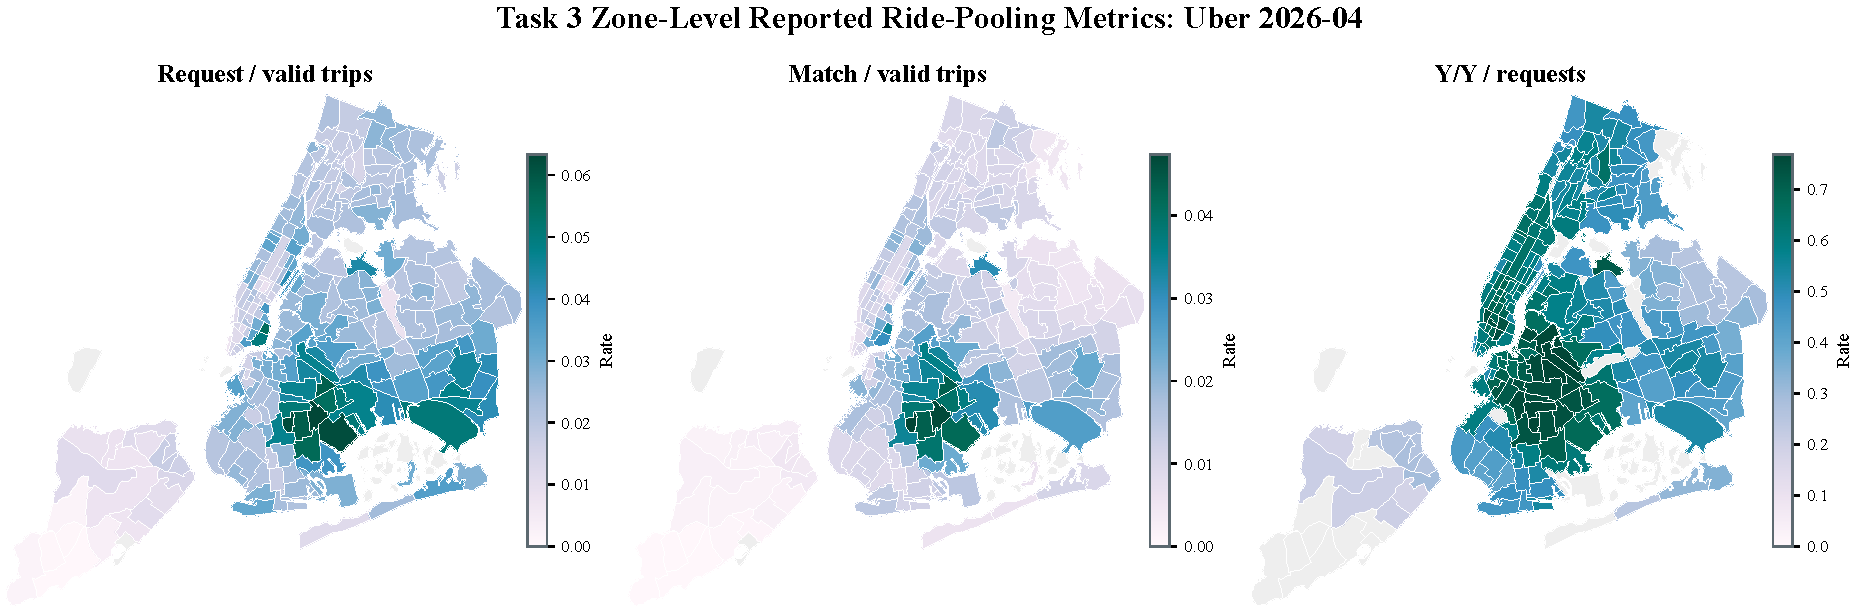
\includegraphics[height=.375\textheight,width=.98\linewidth,keepaspectratio]{04_Results/report_figures/appendix/task3_zone_metrics_2026-04_uber.pdf}\par\vspace{0.3em}
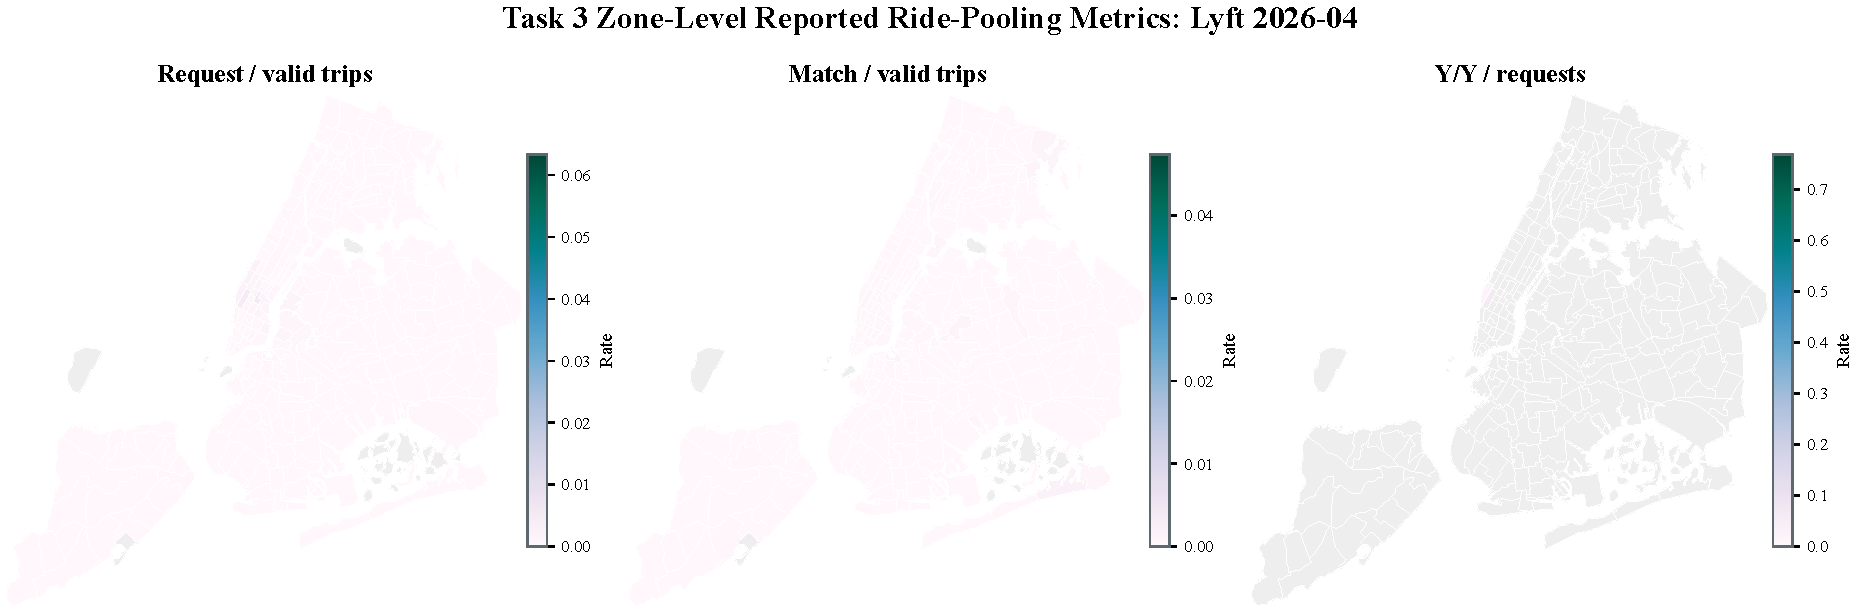
\includegraphics[height=.375\textheight,width=.98\linewidth,keepaspectratio]{04_Results/report_figures/appendix/task3_zone_metrics_2026-04_lyft.pdf}
\captionof{figure}{Zone-level reported ride-pooling metrics in 2026-04. Panels from top to bottom: Uber and Lyft. Gray zones have insufficient sample.}
\end{center}
\clearpage

\begin{center}
\centering
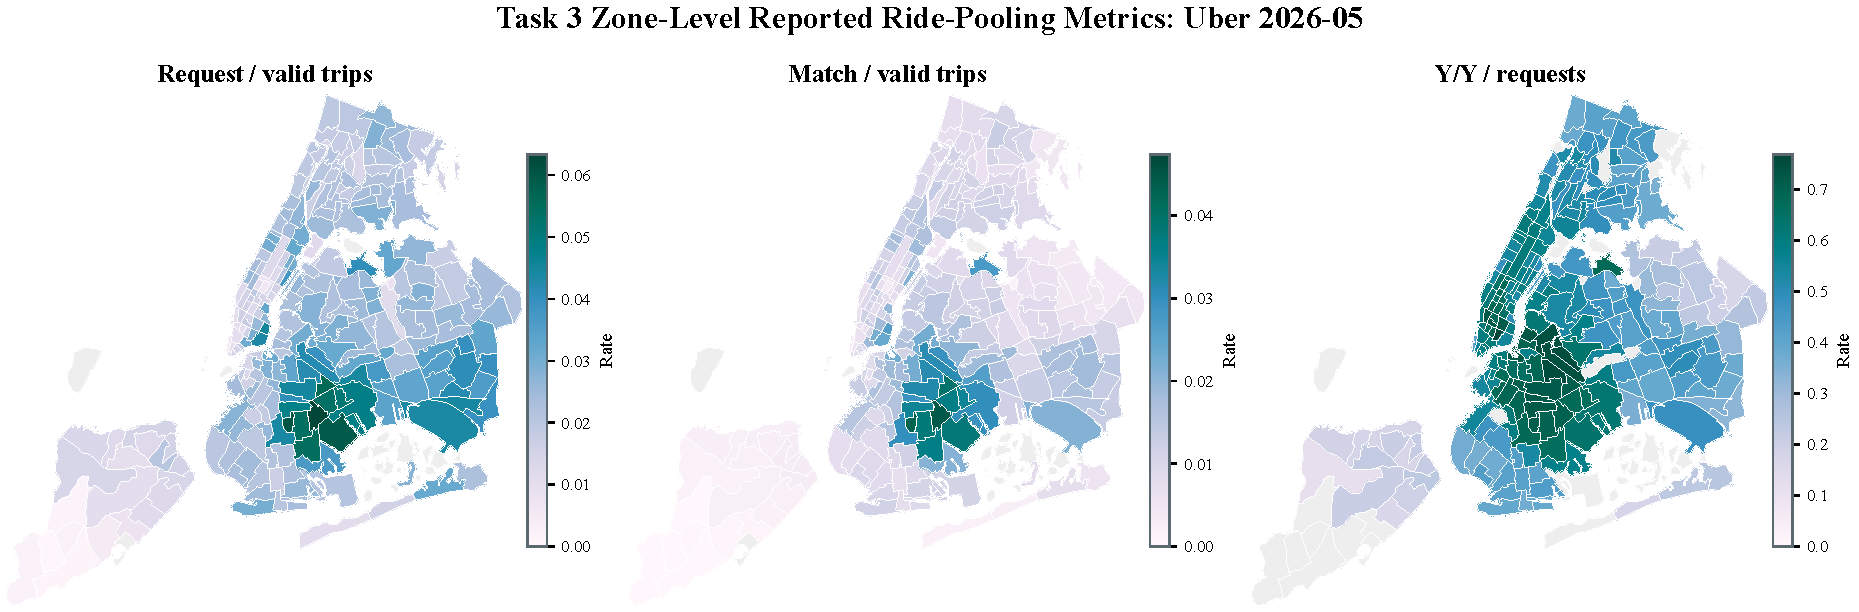
\includegraphics[height=.375\textheight,width=.98\linewidth,keepaspectratio]{04_Results/report_figures/appendix/task3_zone_metrics_2026-05_uber.pdf}\par\vspace{0.3em}
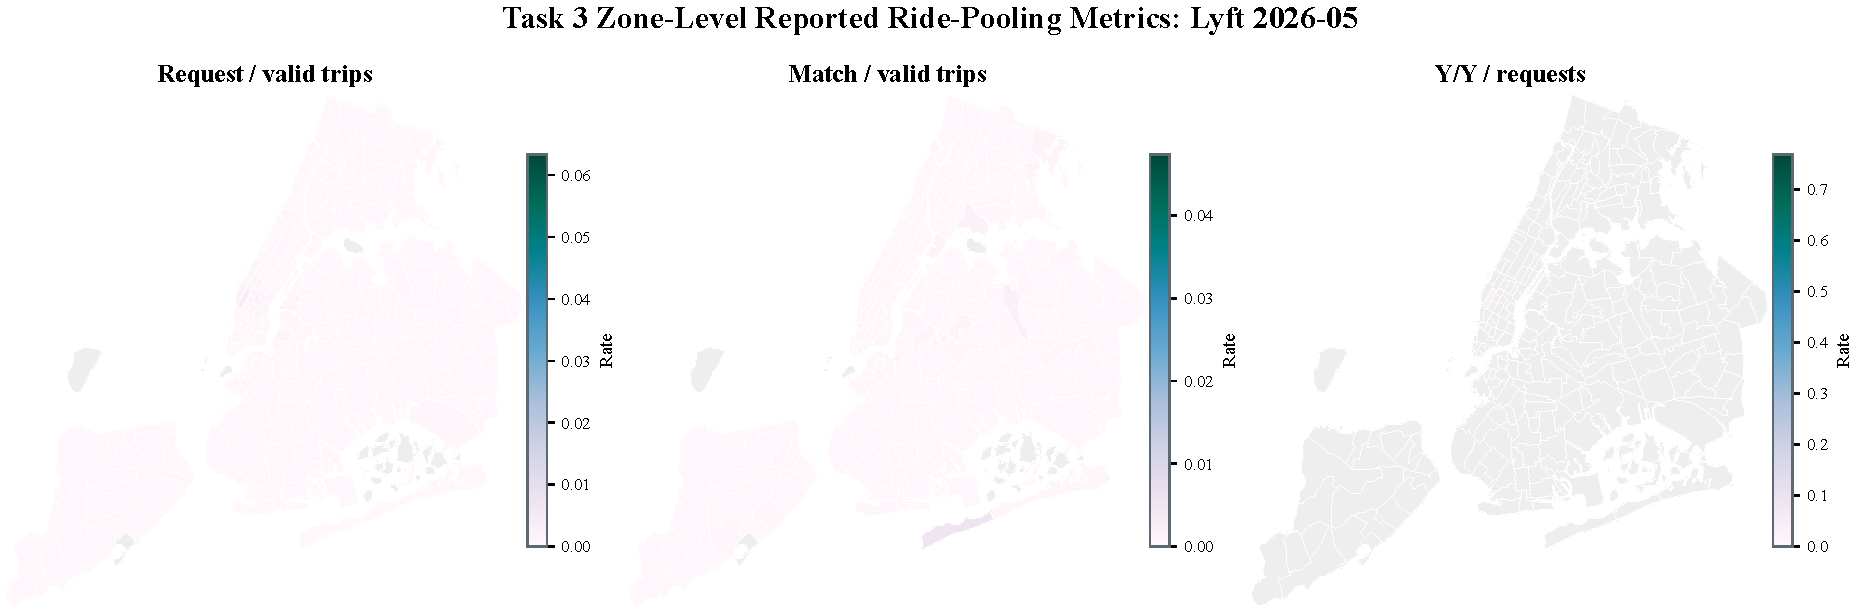
\includegraphics[height=.375\textheight,width=.98\linewidth,keepaspectratio]{04_Results/report_figures/appendix/task3_zone_metrics_2026-05_lyft.pdf}
\captionof{figure}{Zone-level reported ride-pooling metrics in 2026-05. Panels from top to bottom: Uber and Lyft. Gray zones have insufficient sample.}
\end{center}
\clearpage

\subsection{Spatial travel-time differences and reference coverage}
These maps show where supported Uber comparisons are available and how the observed mean travel-time difference varies by pickup zone.

\begin{center}
\centering
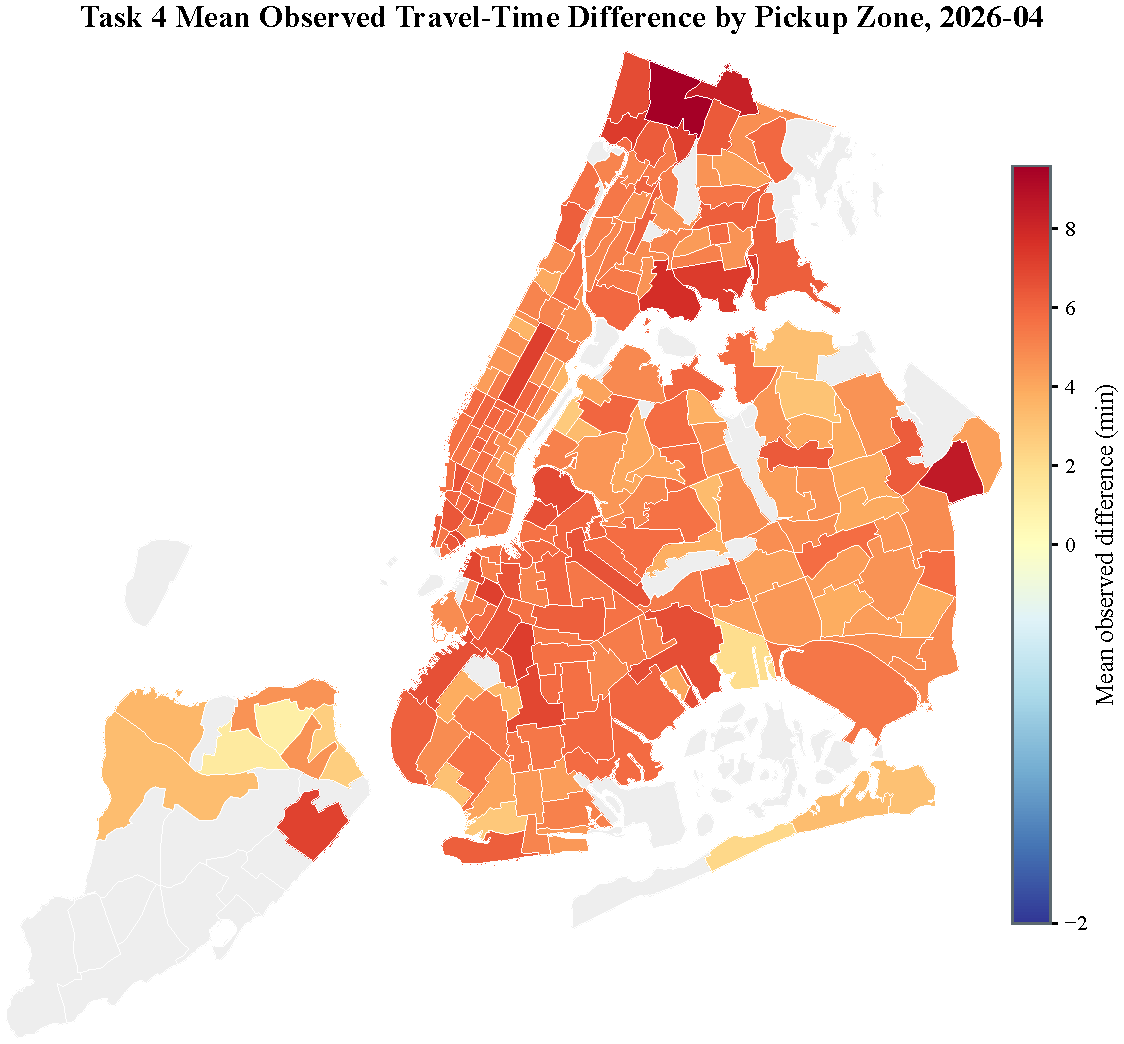
\includegraphics[height=.265\textheight,width=.98\linewidth,keepaspectratio]{04_Results/report_figures/appendix/task4_zone_mean_difference_2026-04.pdf}\par\vspace{0.2em}
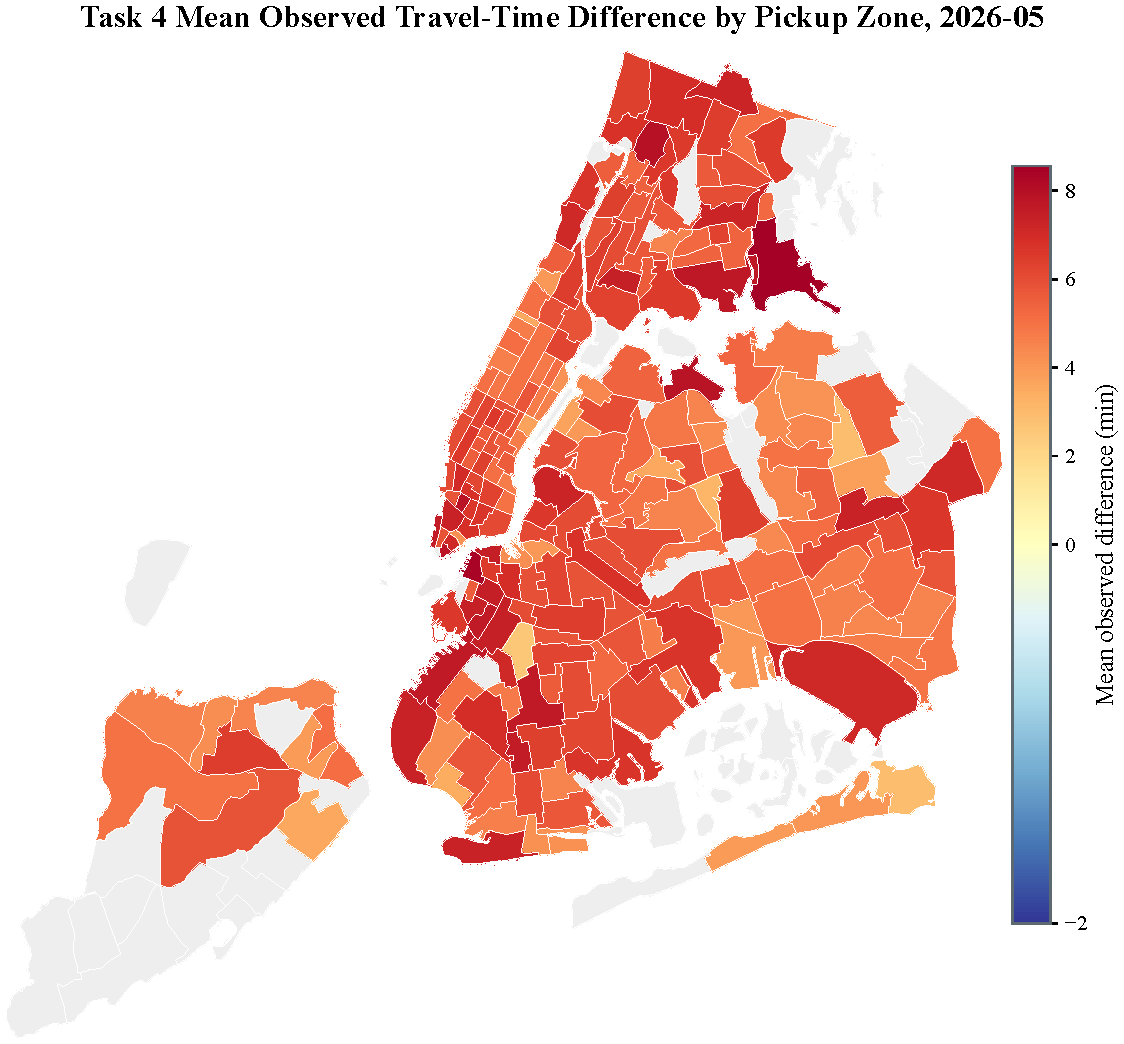
\includegraphics[height=.265\textheight,width=.98\linewidth,keepaspectratio]{04_Results/report_figures/appendix/task4_zone_mean_difference_2026-05.pdf}\par\vspace{0.2em}
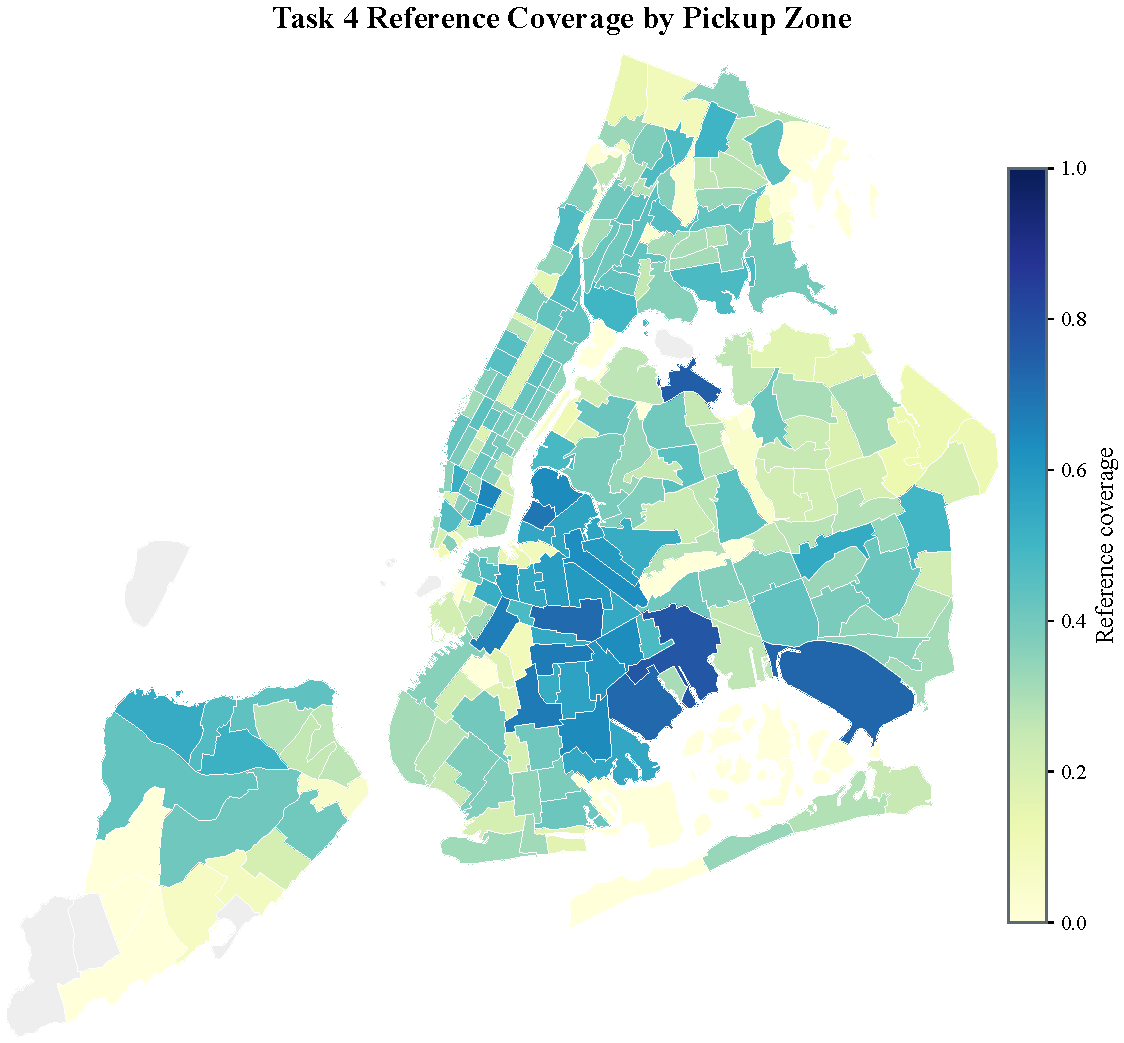
\includegraphics[height=.265\textheight,width=.98\linewidth,keepaspectratio]{04_Results/report_figures/appendix/task4_zone_reference_coverage.pdf}
\captionof{figure}{Spatial travel-time comparison diagnostics for Uber shared trips. Panels from top to bottom: April mean difference, May mean difference, and reference coverage.}
\end{center}

\endgroup

\end{document}
